\documentclass{beamer}

\title{Framework about the inference of sediment contamination level based on zoobenthic community structure}
\author{Feng Gu}
\date{\today}

\begin{document}

\frame{\titlepage}

\begin{frame}
\frametitle{Introduction - Motivation}

Considering the benefits in research, practical and economical aspects, 
there is a motivation to develop \textbf{a sediment contamination level} inference method 
based on the \textbf{zoobenthic community structure}.

% One view is that the two inputs fed into the model may partially represent human activities and 
% ecological reactions. Studying this specific relationship is to reveal how human activities 
% affect the ecological condition, and how to use ecological indicators to infer the human influence.

\begin{figure}
\centering
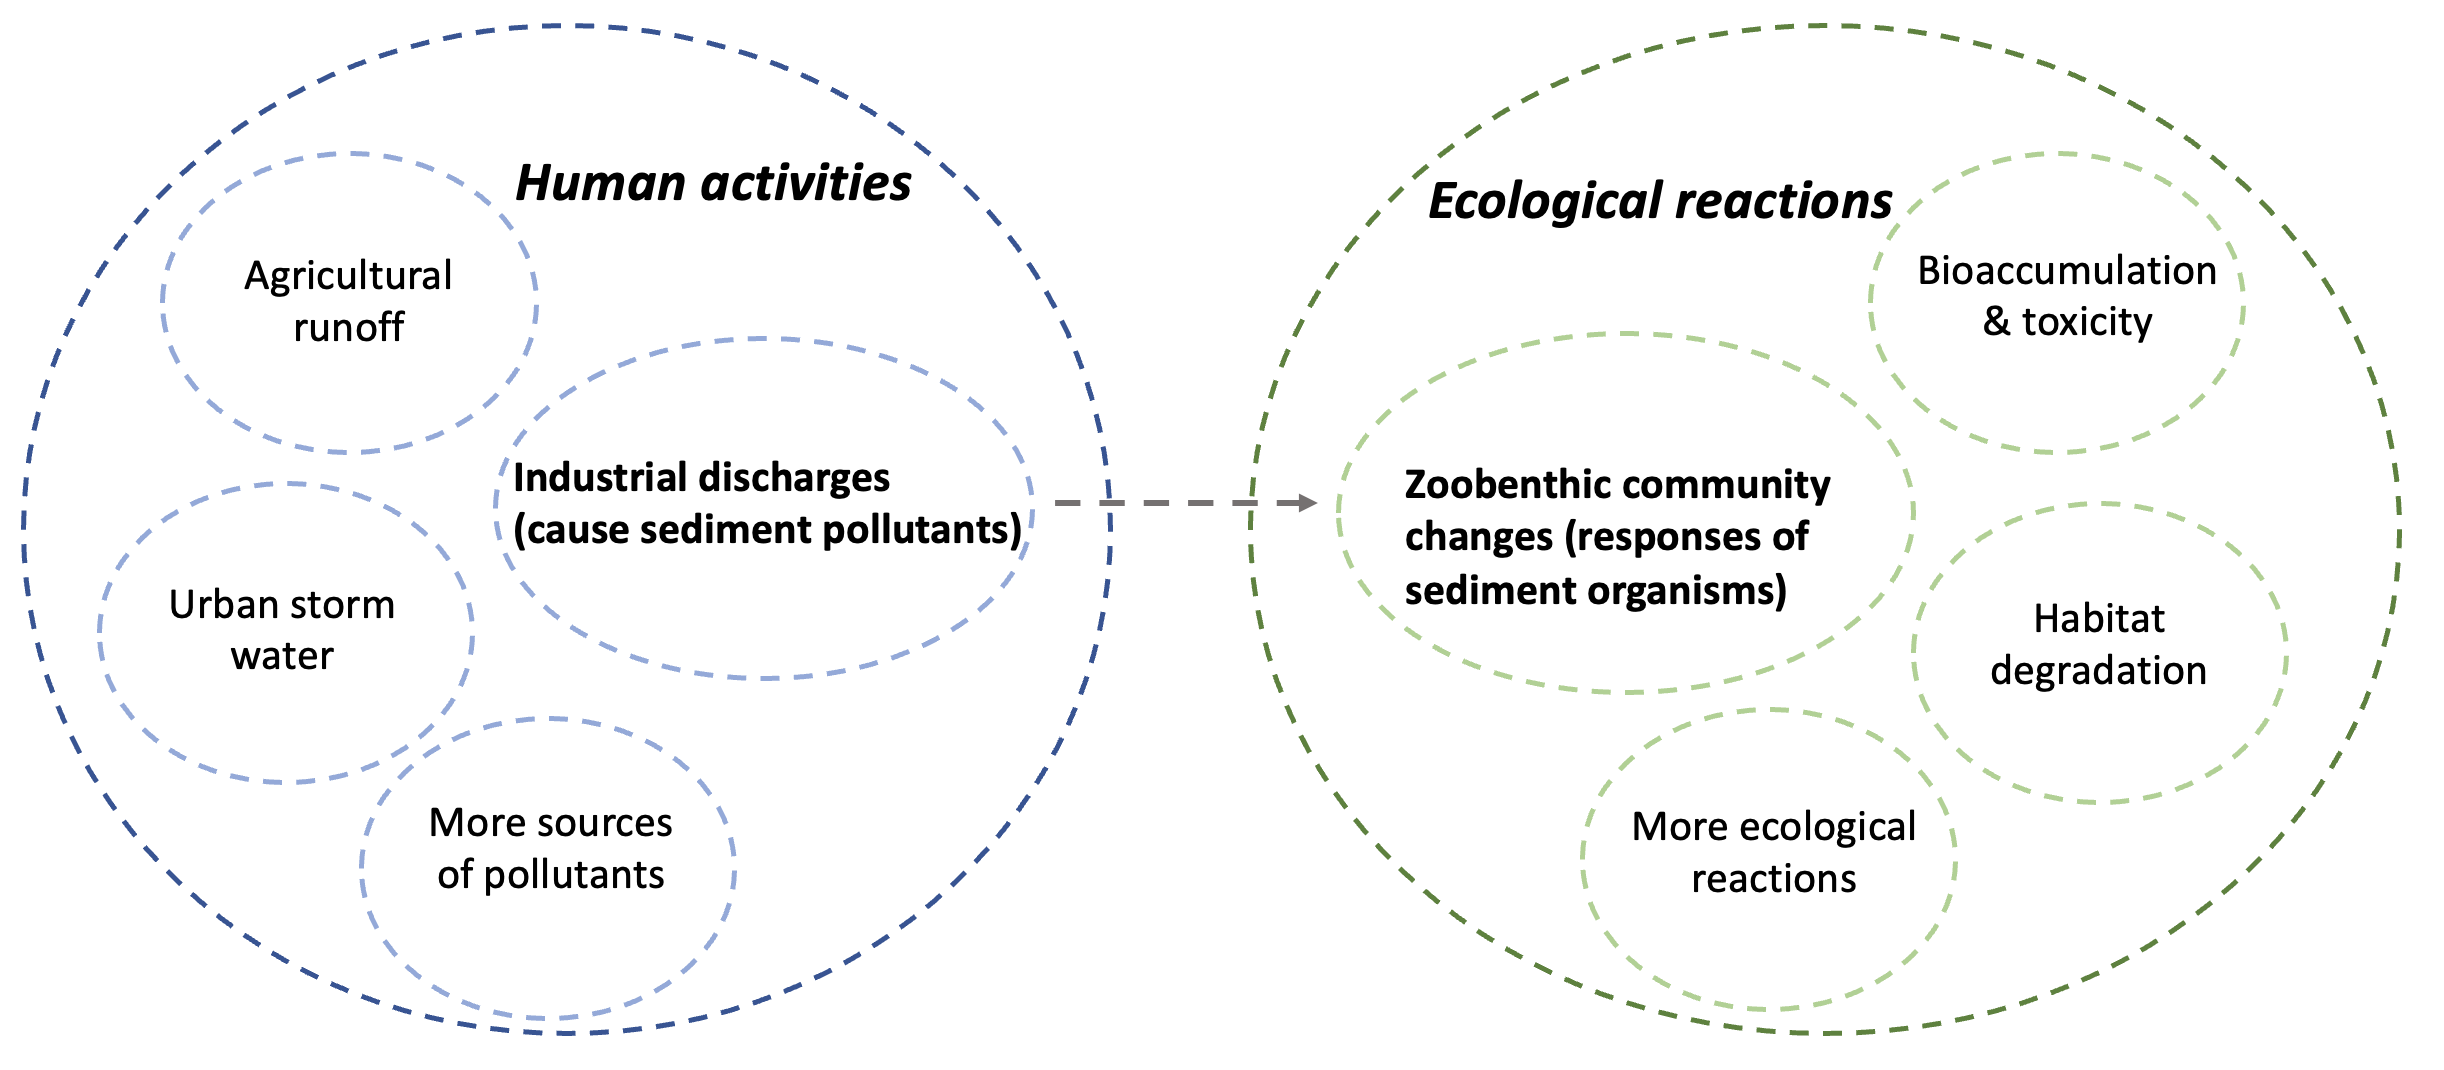
\includegraphics[width=0.8\textwidth]{figures/p1_human_activities_vs_ecological_reactions.png}
\caption{There are relationships between Human activities and ecological reactions}
\end{figure}

\end{frame}

\begin{frame}

\frametitle{Introduction - Problem Statement}
From natural observations, we need to design \textbf{numerical measurements for sediment contamination level and 
zoobenthic community structure} to describe them in numerical terms and 
build a model to infer the relationship between them.

An unignorable fact is that
\textbf{the zoobenthic community structure is influenced by environmental factors},
which must be controlled for its different levels of influence to improve the inference accuracy.


\begin{figure}
\centering
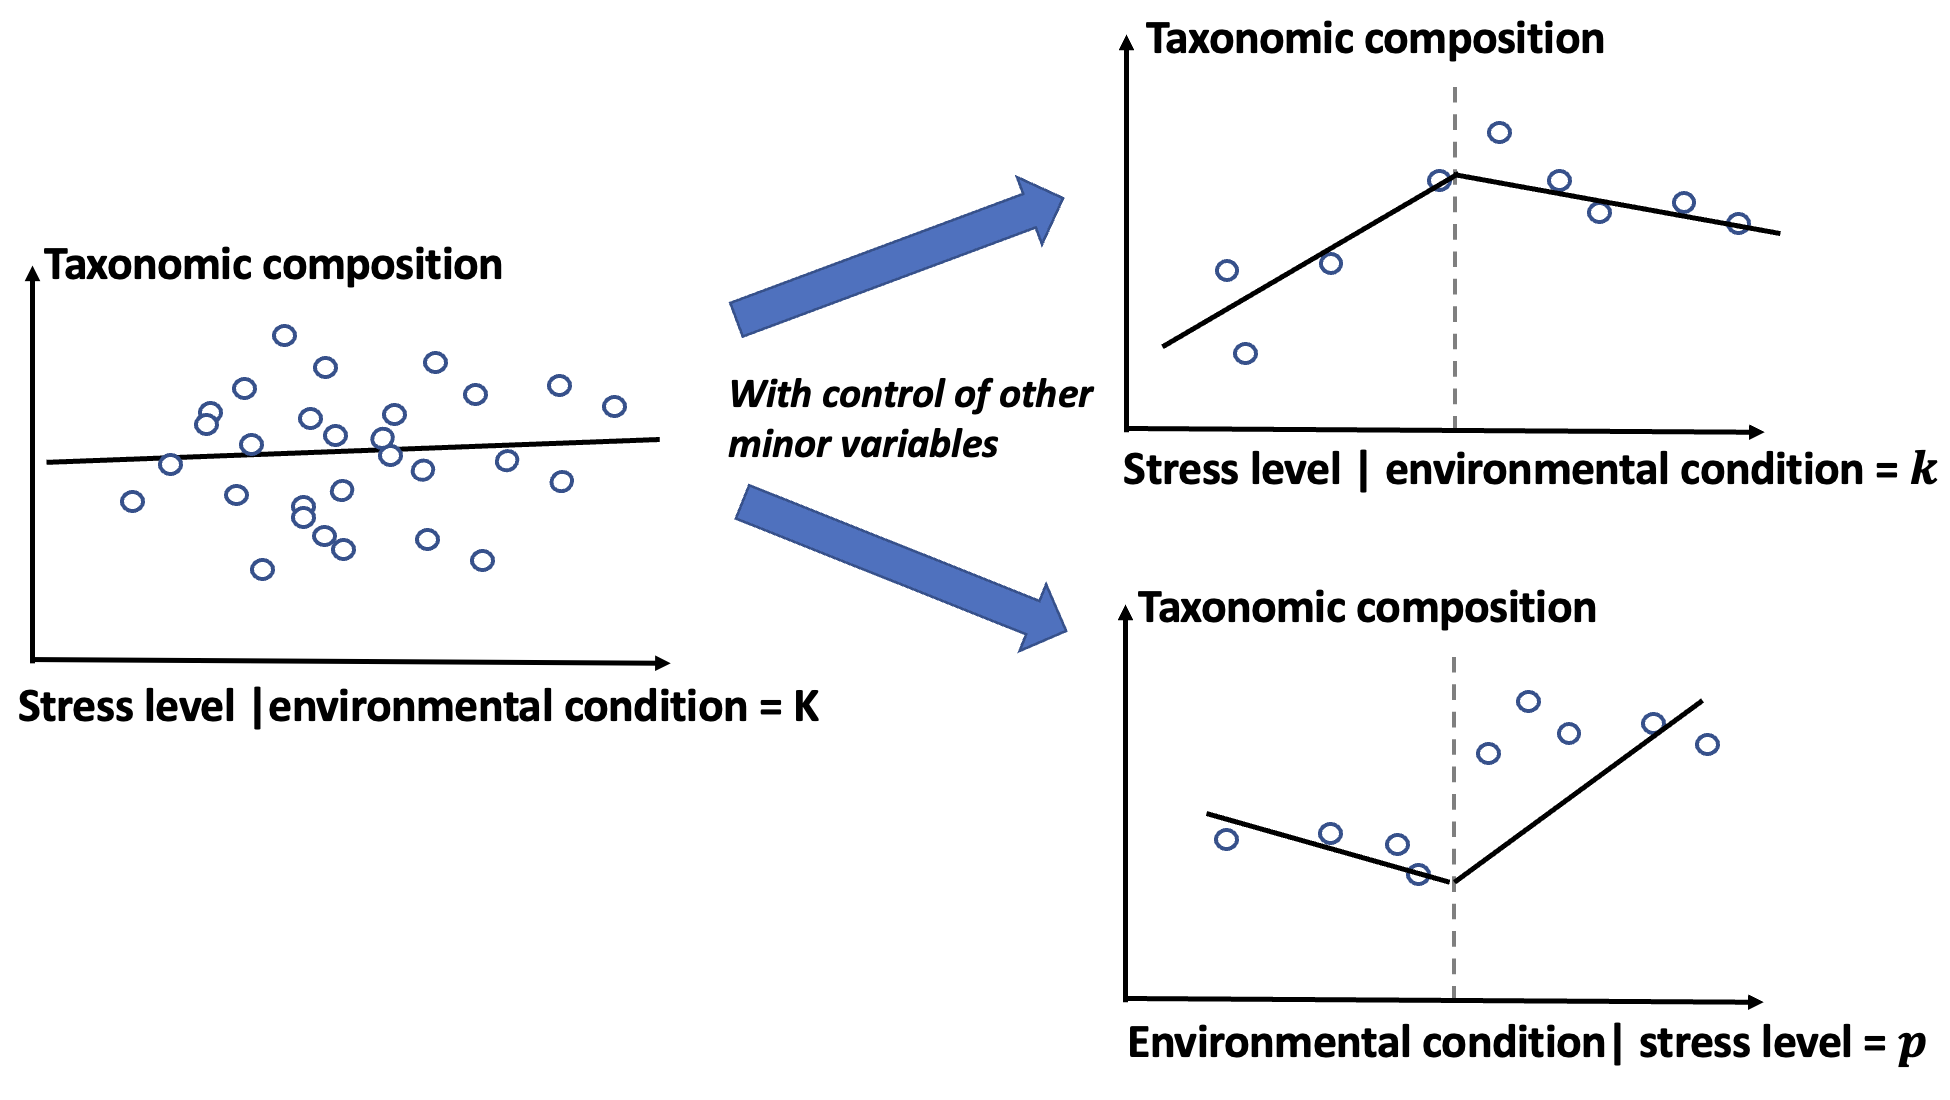
\includegraphics[width=0.7\textwidth]{figures/p2_control_vs_no_control_of_environment.png}
\caption{Environmental factors influence zoobenthic community structure}
\end{figure}

\end{frame}


\begin{frame}
\frametitle{Data Collection}
The data was prepared by Prof. Jan and his team, includes three 
types of data collected from the Lake Huron-Erie Corridor:

\begin{itemize}
    \item Chemical data (\(m \times 30\)), including: metal concentrations, PCBs and PAHs from factors or mining.
    \item Environmental data (\(m \times 5\) or \(m \times 6\)), including: temperature, pH, dissolved oxygen, etc.
    \item Zoobenthic macroinvertebrates data (\(m \times 16\)), including: selected organisms living in the sampled sediment, 
    where chemical data was collected.
\end{itemize}

Three separated matrices with shared identical row indices,
where each row represents a site sampled at a specific time and location.

\end{frame}

\begin{frame}
\frametitle{Overview to data operation rules along the analysis}

The three data matrices are merged into a single matrix by row indices,
later processes that bring new information to each site will be merged into this single matrix by row indices as well.


\begin{figure}
\centering
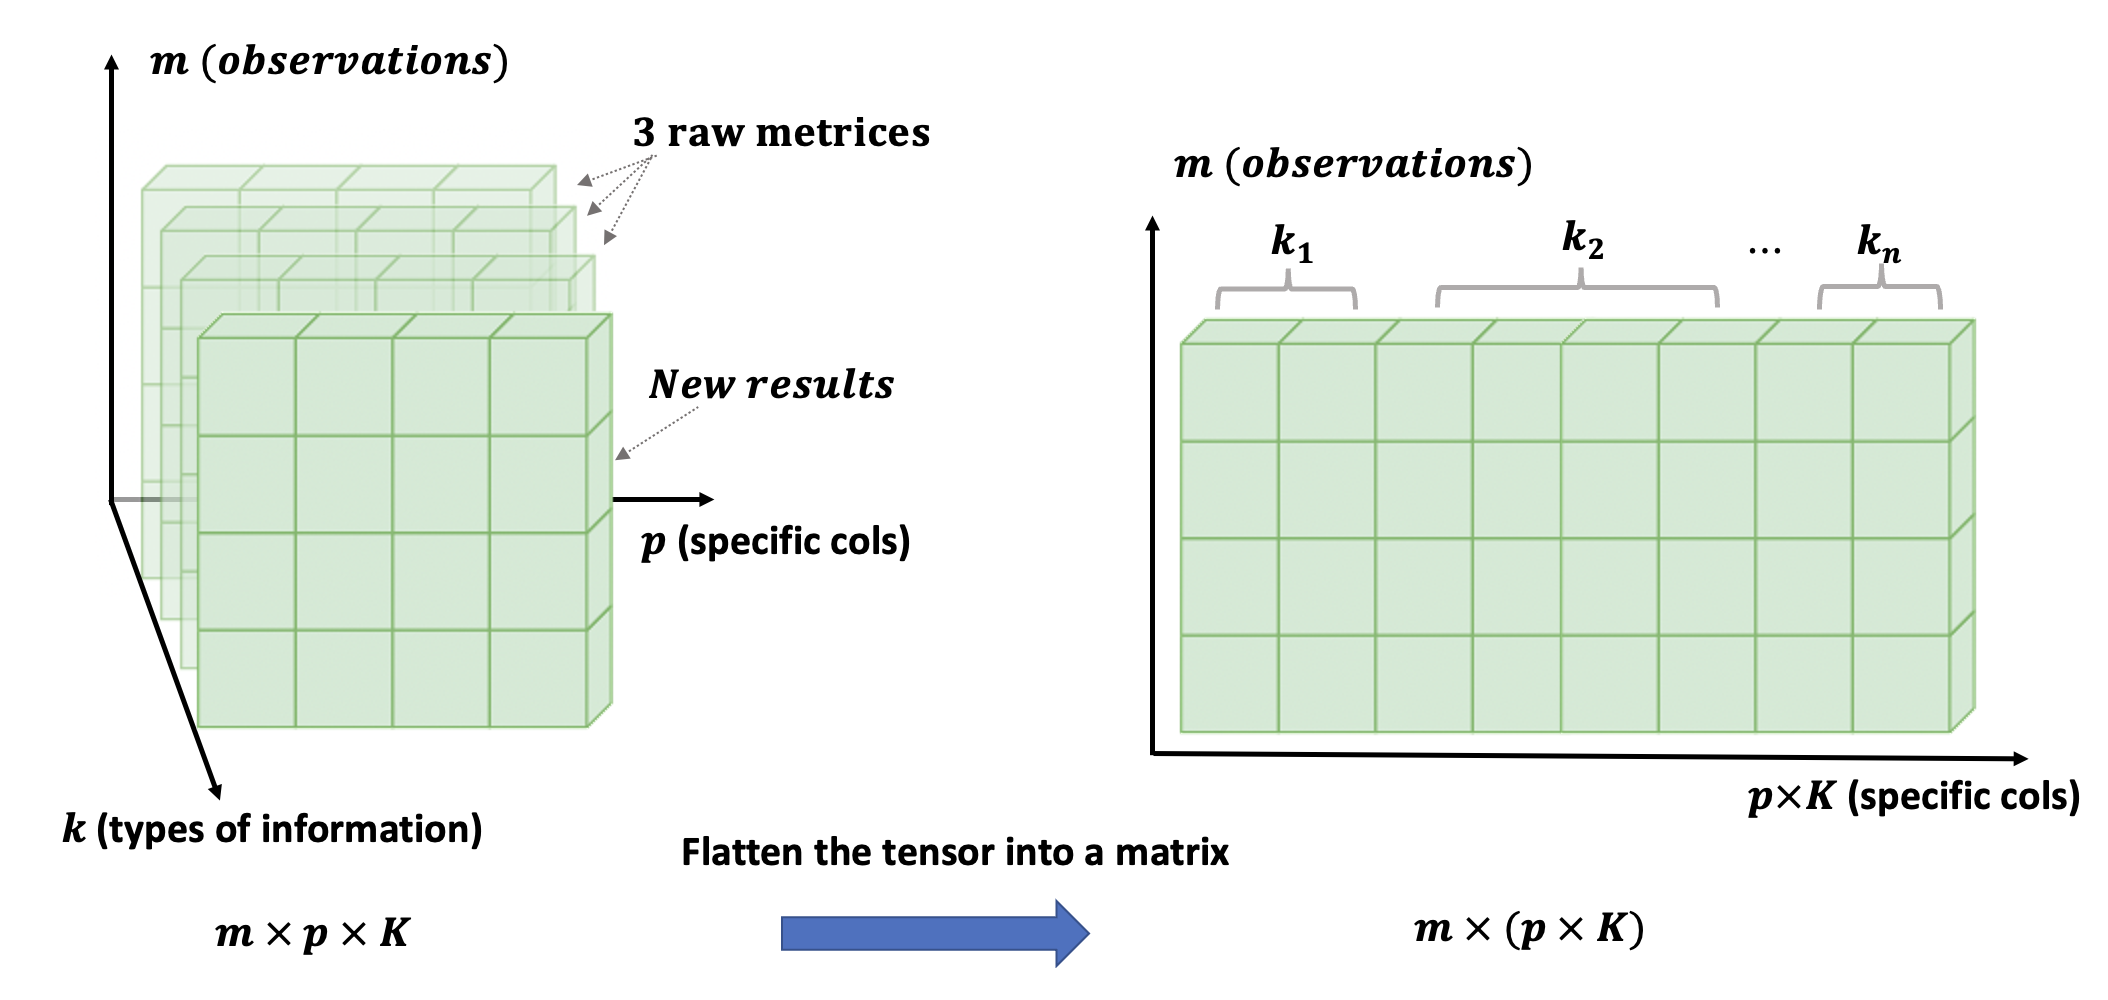
\includegraphics[width=\textwidth]{figures/p4_rules_for_data_operation.png}
\caption{Data operation rules along the analysis}
\end{figure}

\end{frame}

\begin{frame}
\frametitle{Instance of the data operation rules}

\begin{figure}
\centering
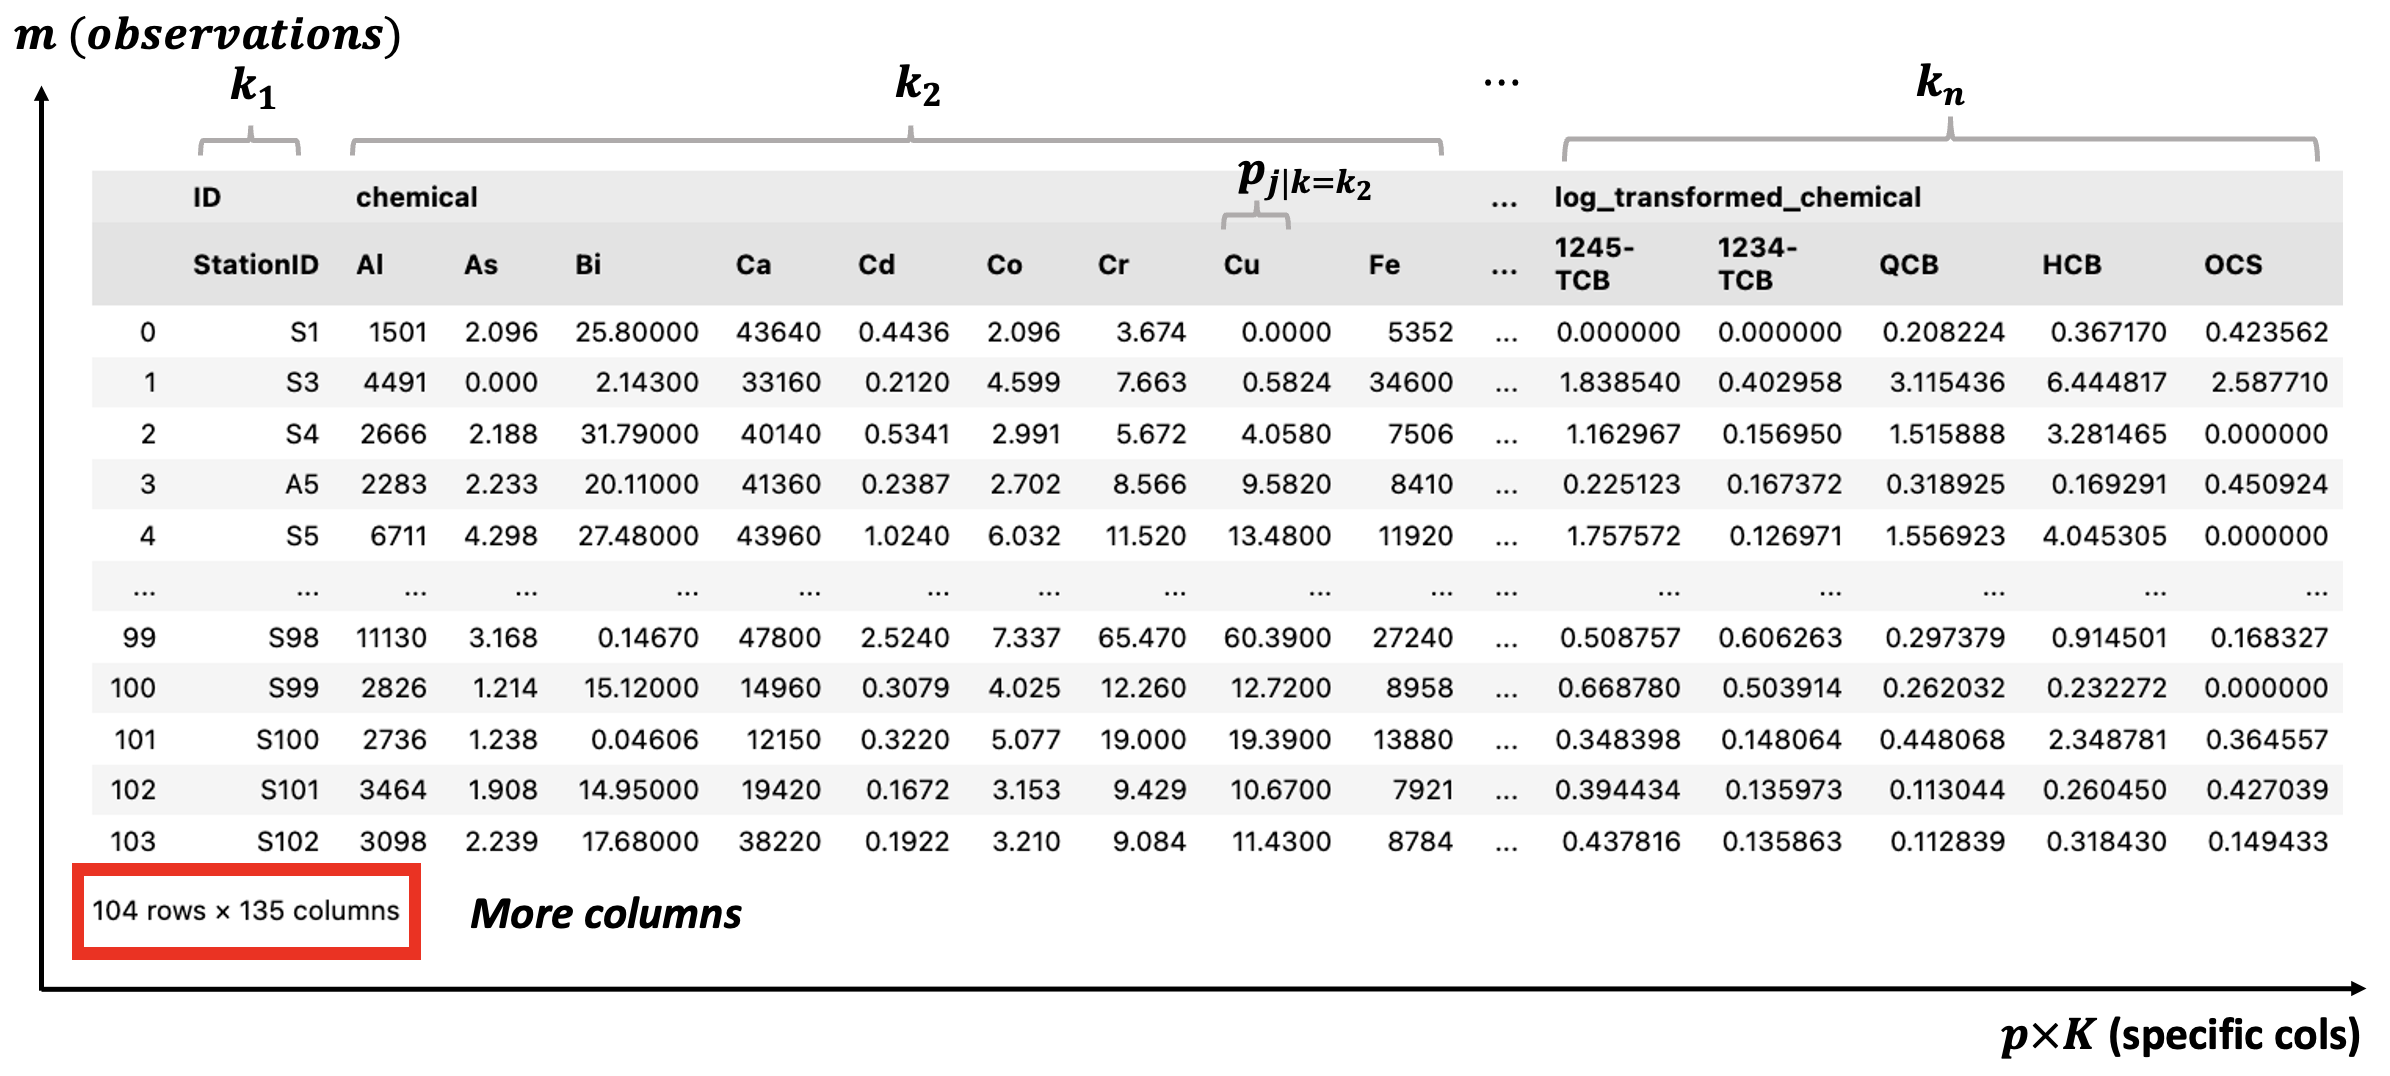
\includegraphics[width=\textwidth]{figures/p5_application_data_rules.png}
\end{figure}

It does not directly relates to the inference model, but it makes data operation easier and smoother
to accelerate the analytical process.
\end{frame}

\begin{frame}
\frametitle{Framework of the analysis}
\begin{figure}
\centering
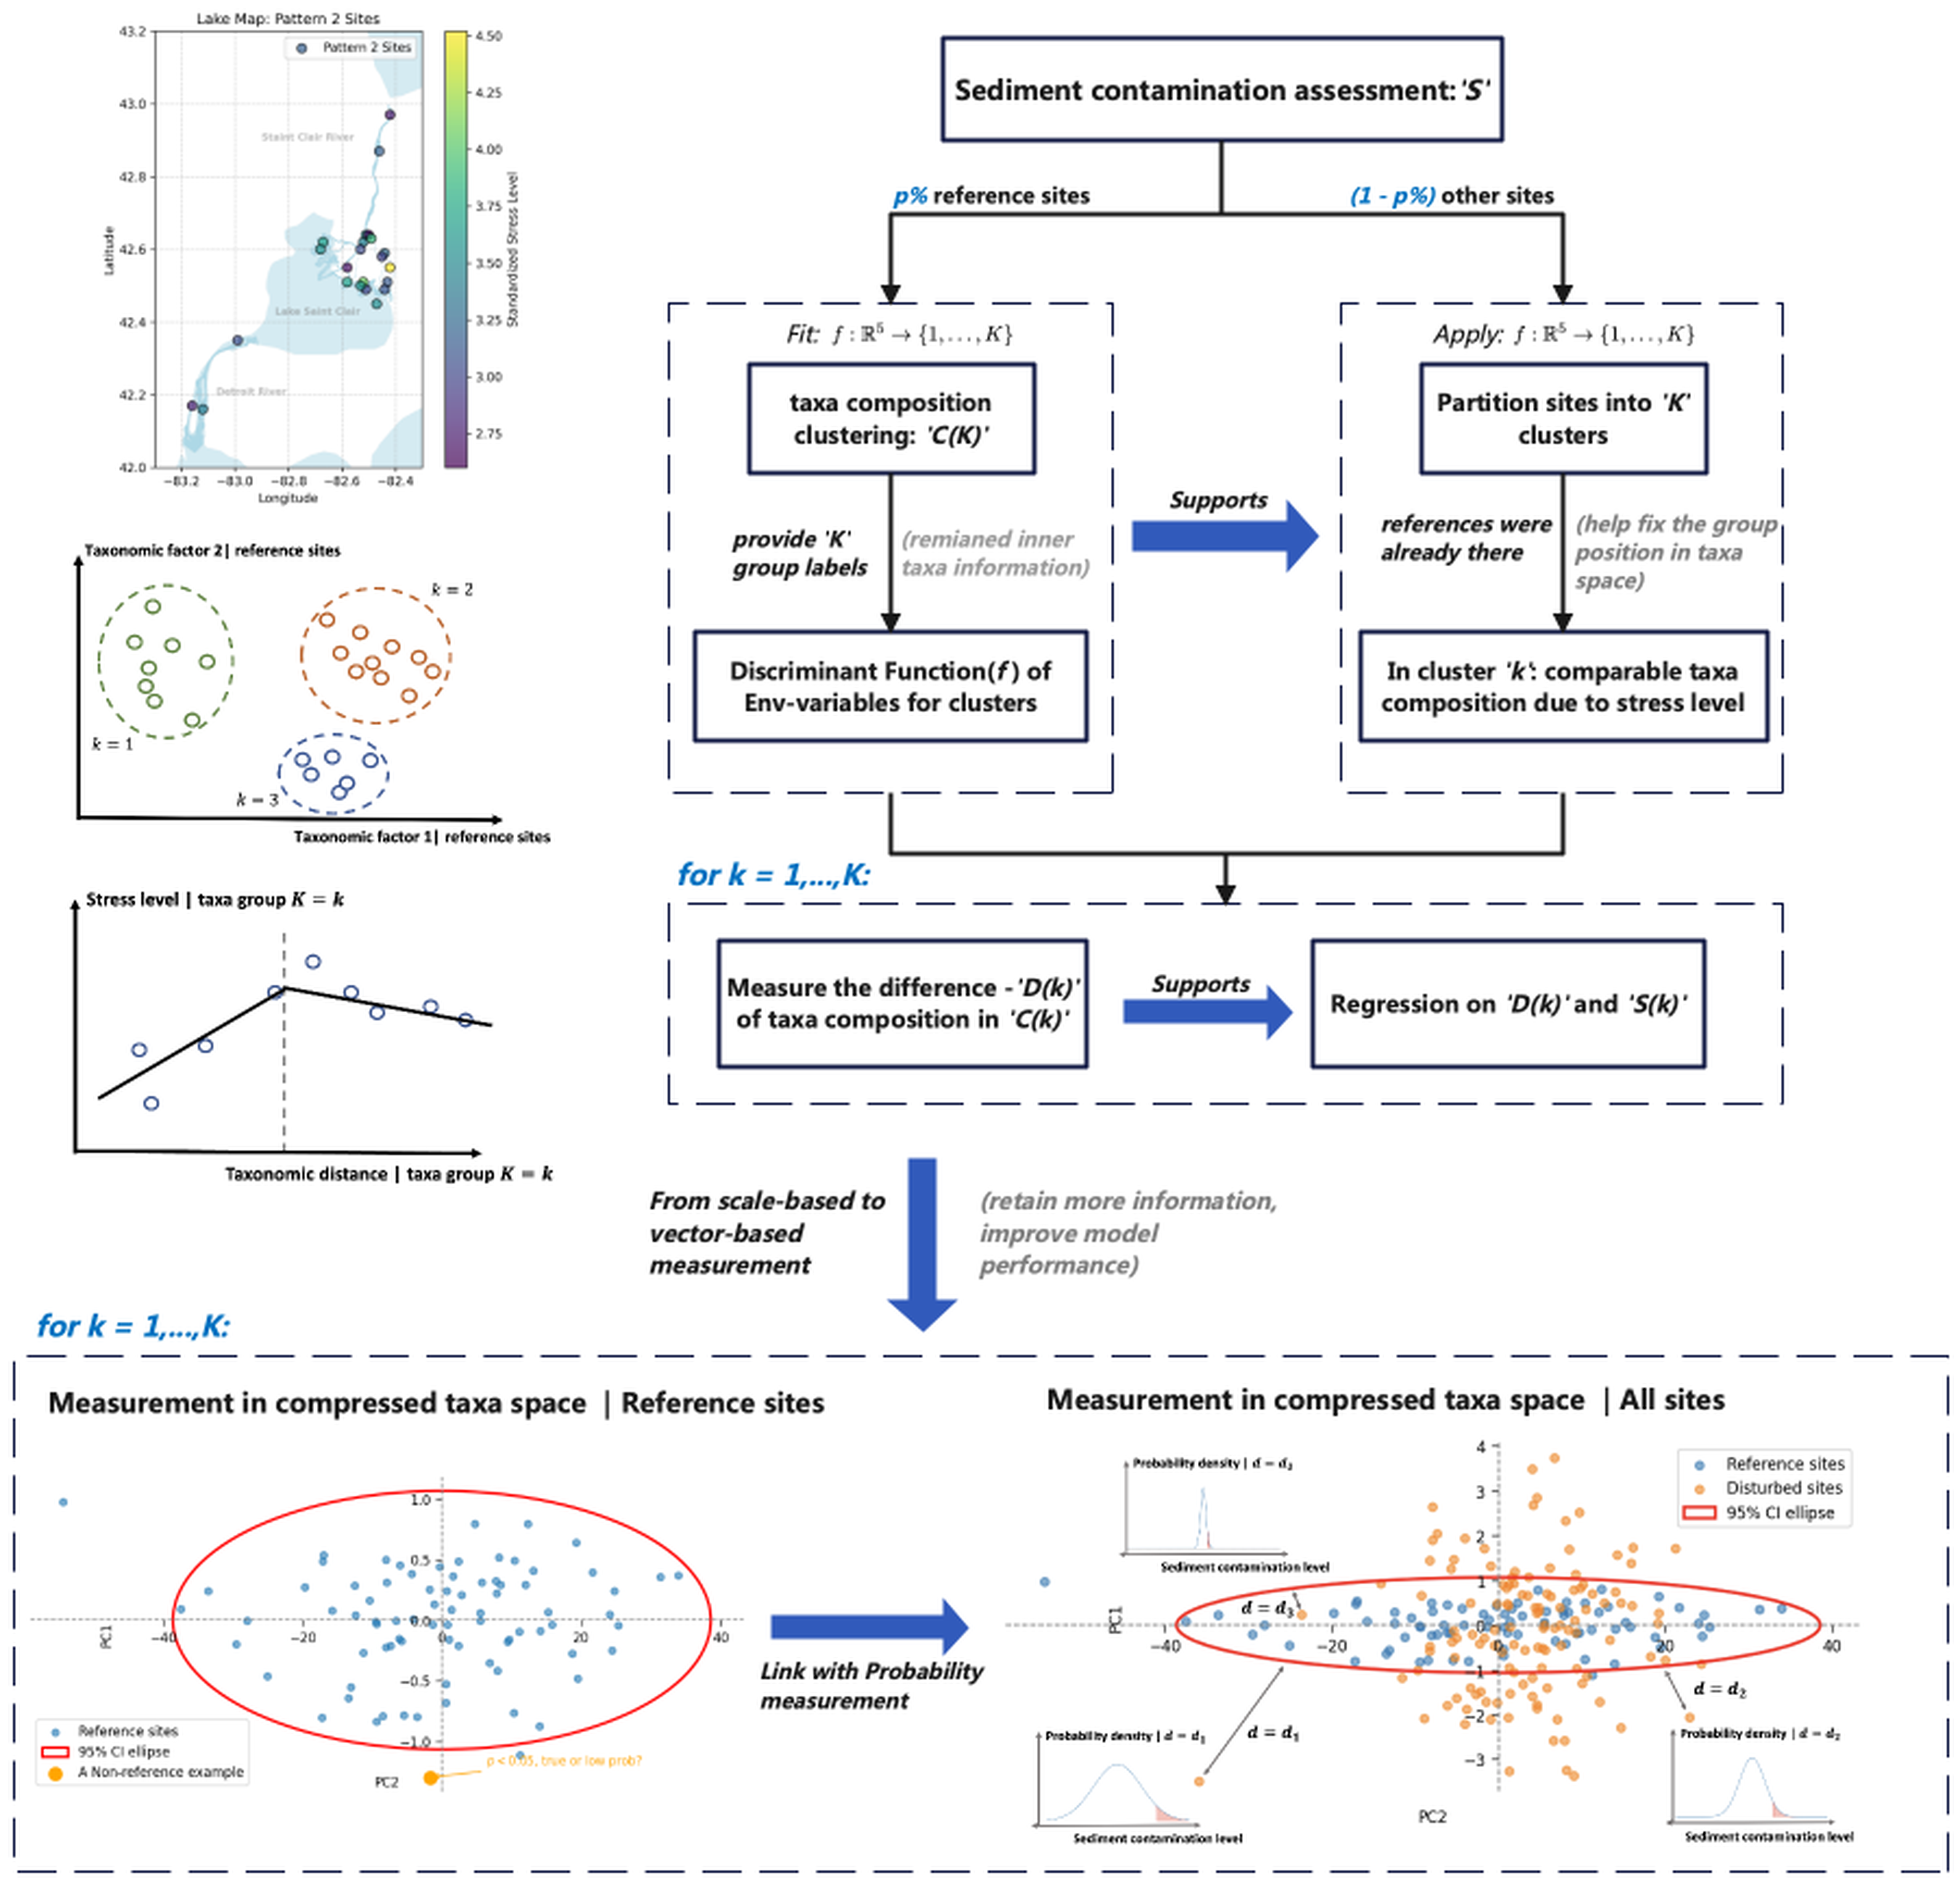
\includegraphics[height=0.85\textheight,keepaspectratio]{figures/p6_workflow_of_general_workframe.png}        
\end{figure}
\end{frame}

\begin{frame}
\frametitle{Sediment Contamination Level Assessment}

Let $\mathbf{X} \in \mathbb{R}^{n \times p}$ be the log-transformed chemical data. Apply PCA:
\[
\mathbf{Z} = \mathbf{X} \mathbf{W}
\]
where $\mathbf{W}$ contains loadings of $k$ selected PCs. \textbf{Normalize each PC}:
\[
\tilde{\mathbf{z}}_j = \frac{\mathbf{z}_j - \min(\mathbf{z}_j)}{\max(\mathbf{z}_j) - \min(\mathbf{z}_j)}
\]
The contamination score for sample $i$:
\[
S_i/ \text{SumReal}_i = \sum_{j=1}^k \alpha_j \tilde{z}_{ij}
\]
where $\alpha_j$ reflects the direction and importance of each PC.

\end{frame}


\begin{frame}
\frametitle{Pick up references for control of sediment contamination level}
Assuming the least stressed sites are references and they were \textbf{not or minimally influenced} by human activities,
vice versa.

\[
\mathcal{R} = \{ i : S_i \leq Q_{p\%}(S) \}, \quad
\mathcal{D} = \{ i : S_i \geq Q_{(100-p)\%}(S) \}
\]
where $S_i$ is the stress score for site $i$, and $Q_{p\%}(S)$, $Q_{(100-p)\%}(S)$ are the $p$-th and $(100-p)$-th percentiles.

% \vspace*{.6 cm}

These references will support building a purely tidy model that predicts what
a pristine taxa composition should be given a specific set of environmental conditions
\footnote{
Notice the references-environmental distribution, a uniform or proportional to the real world distribution
is better for capturing real world relationships}.

\end{frame} 

\begin{frame}
\frametitle{Pick up references for control of sediment contamination level}

\begin{figure}
\centering
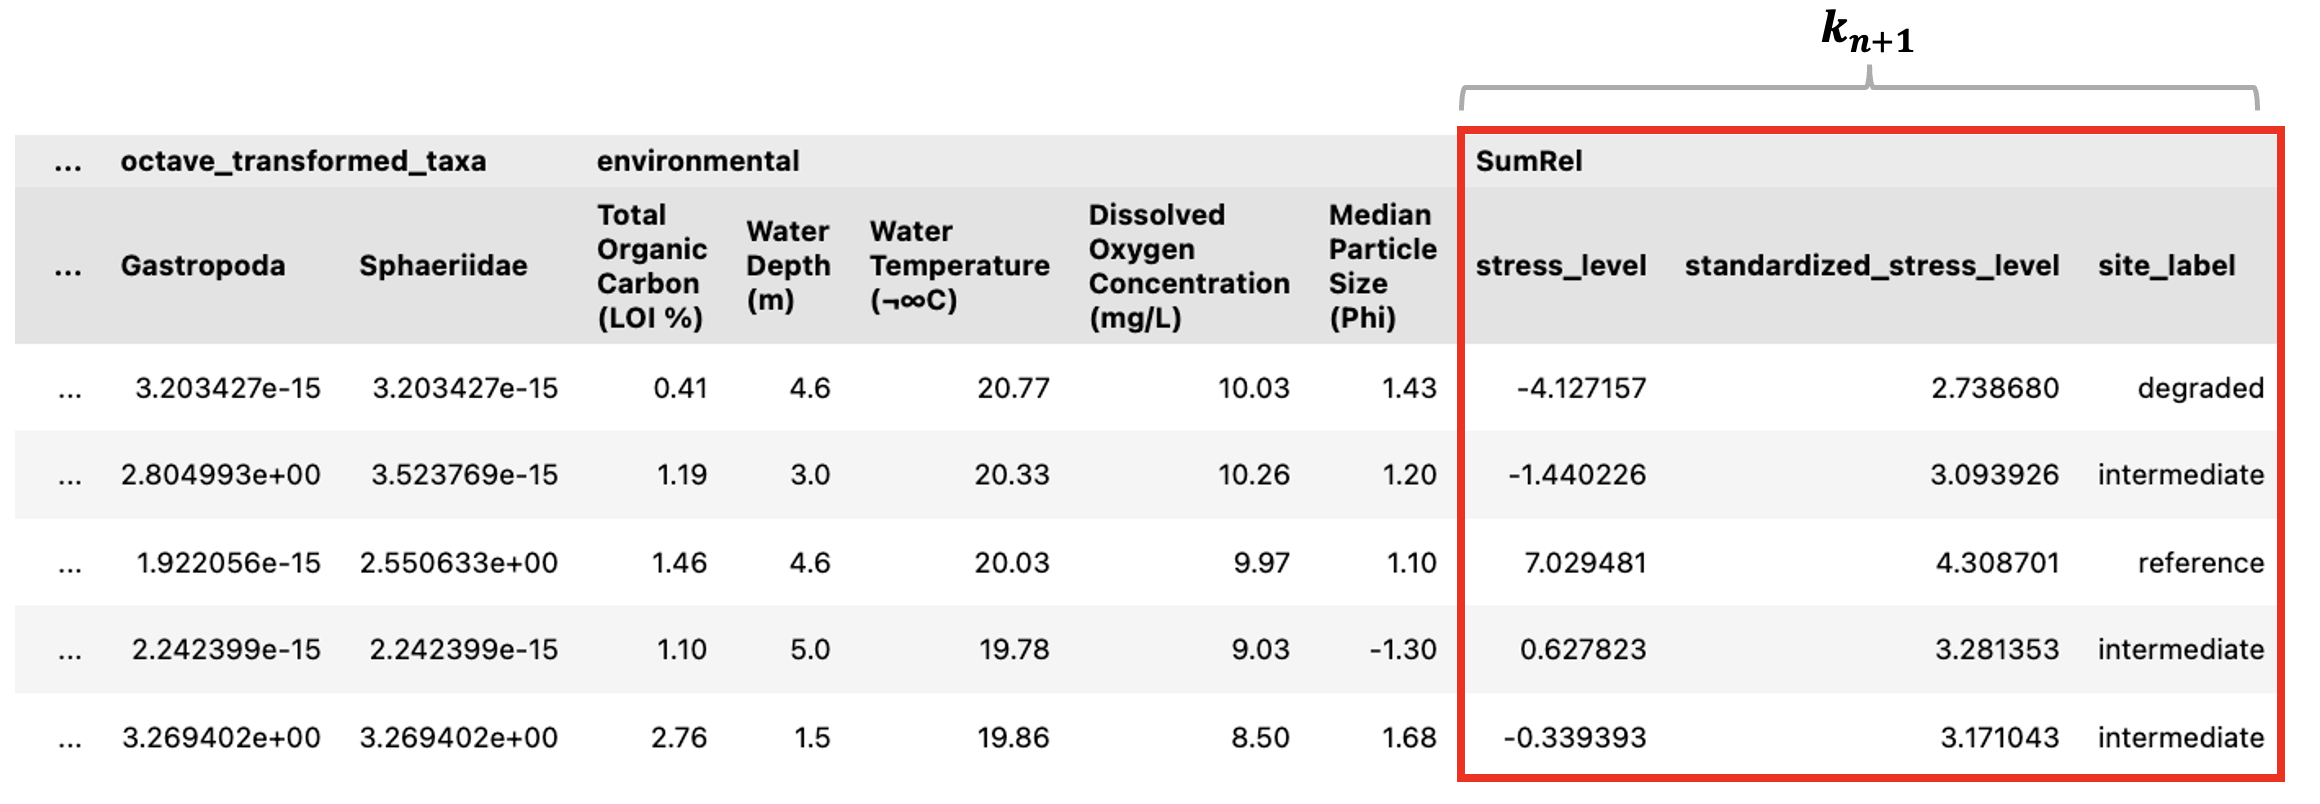
\includegraphics[width=\textwidth]{figures/p8_added_stress_scores.png}
\caption{New stress scores information added to the data matrix}
\end{figure}

\end{frame}

\begin{frame}
\frametitle{Determine how environment shapes the taxa composition}

This reference sites have taxa composition that were only shaped by the environment, good 
for exploring how environment determines taxa composition with the control of human impacts.

However, \textbf{5 environmental factors are not enough to explain the taxa composition measured by 16 taxa},
only a poor model can be built on them. 
But explaining limited information of the taxa composition may be good,
like their clustering patterns \(C_K\).

\[
\mathcal{F}: R^{m \times 5} \to R^{m \times 16}, \quad \text{which is not good}
\]

\[
\mathcal{F}: R^{m \times 5} \to C_K^{m \times 1}, \quad \text{which may be good}
\]

The \(C_K^{m \times 1}\) is the clustering label of each site, confined information of its taxa composition.

\end{frame}

\begin{frame}
\frametitle{Clustering on the taxa composition of references}

\begin{center}
        \parbox{0.95\linewidth}{%
            Let $\mathcal{R}$ be the set of reference sites, each with taxa composition $\mathbf{y}_i \in \mathbb{R}^t$. Cluster $\{\mathbf{y}_i : i \in \mathcal{R}\}$ into $K$ groups $\mathcal{C}_1, \ldots, \mathcal{C}_K$:
            \[
            \mathcal{R} = \bigcup_{k=1}^K \mathcal{C}_k, \qquad \mathcal{C}_k \cap \mathcal{C}_l = \emptyset \text{ for } k \neq l
            \]
            Each $\mathcal{C}_k$ contains sites with similar taxa compositions.
        }
\end{center}

\begin{figure}
\centering
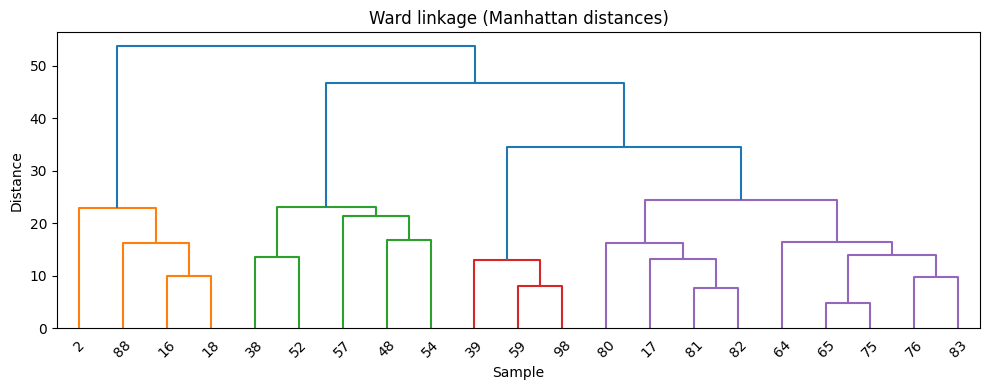
\includegraphics[width=\textwidth]{figures/p10_clustering_results.png}
\end{figure}

\end{frame}

\begin{frame}
\frametitle{Fit Discriminant Function of environmental factors for clustering labels}
\begin{center}
    \parbox{0.95\linewidth}{
        Let $\mathcal{C}_1, \ldots, \mathcal{C}_K$ be resulted taxa cluster labels.
        For each site $i$, let $\mathbf{e}_i$ be its environmental variables.
        \textcolor{blue}{Fit} a discriminant function of environmental variables for cluster labels on the \(p\%\) reference sites:
        \[
        \mathcal{F}: e_{i}^{(1 \times 5)} \mapsto \mathcal{\hat C}_{i, k}, \quad i \in \mathcal{R}, k \in \{1, \ldots, K\}
        \]
        }
\end{center}

\textcolor{blue}{Apply} $\mathcal{F}$ to rest (\(1 - p\%\)) sites to group them into the \(K\) clusters,
where \textcolor{blue}{reference sites were already assigned} after the fitting stage.

\end{frame}

\begin{frame}
\frametitle{Apply Discriminant Function of environmental factors for clustering labels}

\begin{figure}
\centering
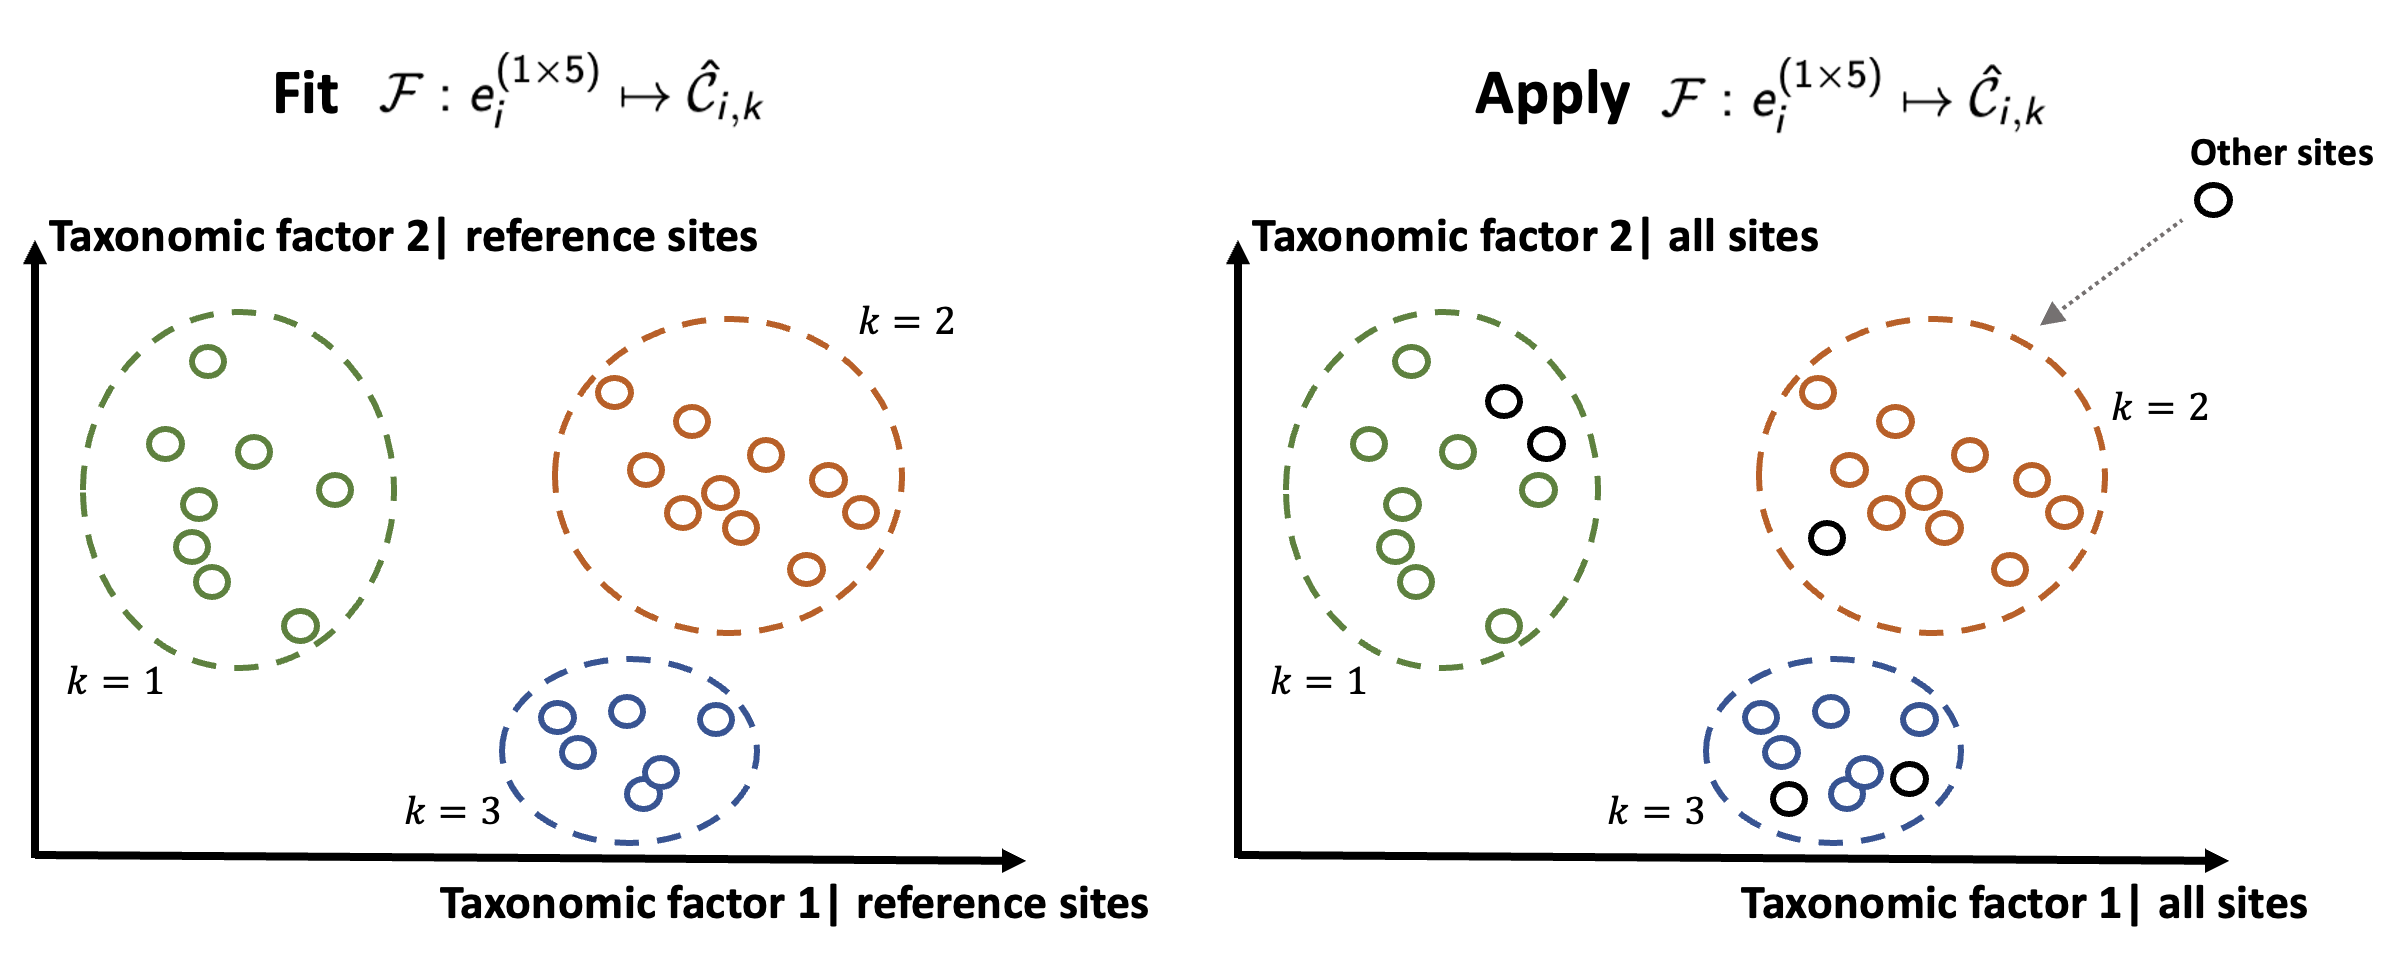
\includegraphics[width=\textwidth]{figures/p12_fit_apply_discriminant_function.png}
\caption{Discriminant function results on the references and rest sites}
\end{figure}

\end{frame}

\begin{frame}
\frametitle{Measure the distance between each site to the references in each cluster}

In each cluster, the references are of the ideal taxa composition, and the rest sites are 
not, this \textcolor{blue}{difference in taxa composition} between them
should be caused by human activities - stress level.

\begin{figure}
\centering
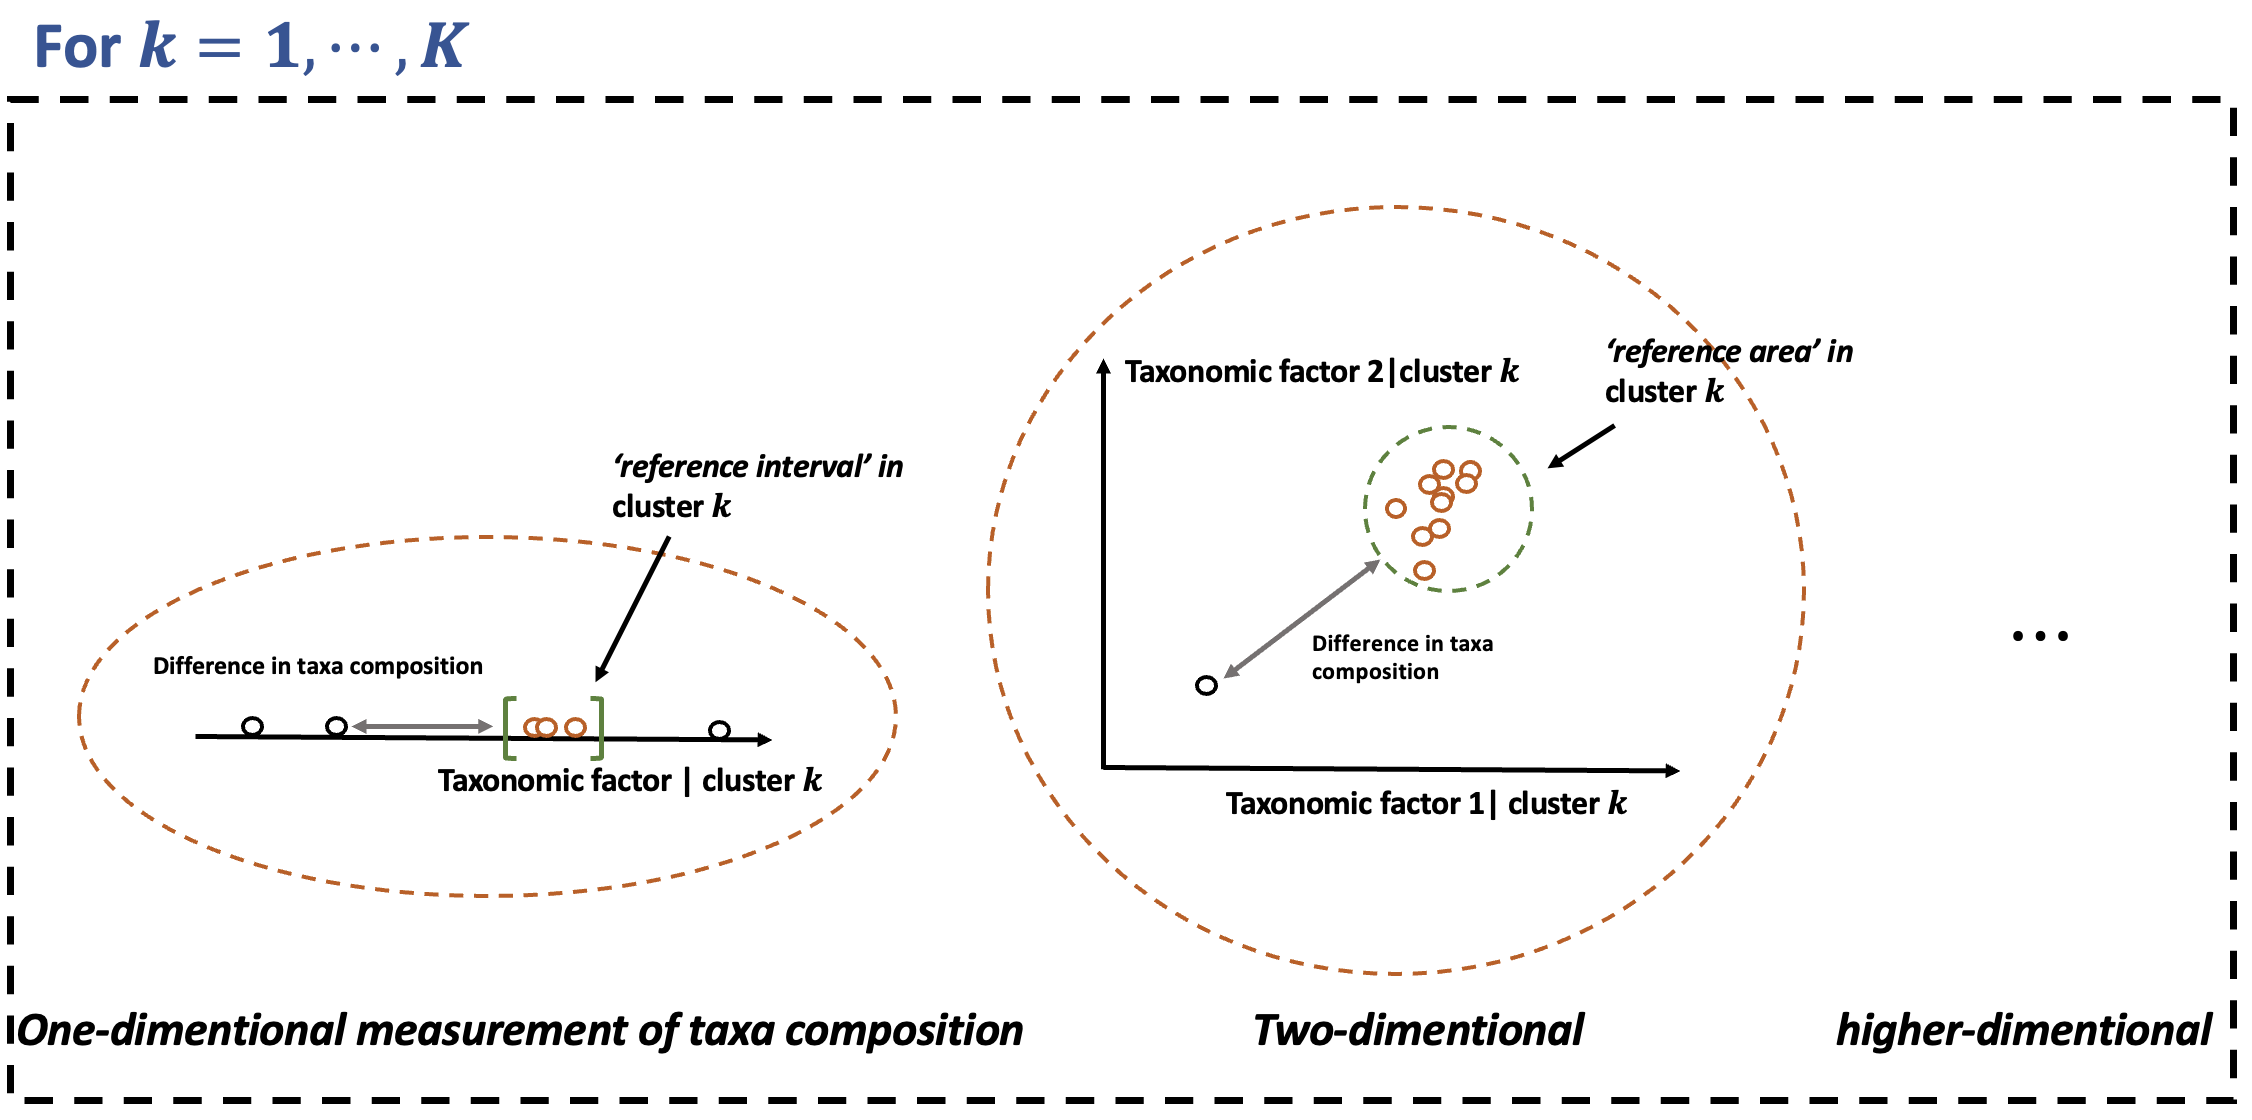
\includegraphics[width=\textwidth]{figures/p_14_differences_in_taxa_across_clusters.png}
\end{figure}

\end{frame}

\begin{frame}
    \frametitle{Details in the the one-dimensional taxa difference measurements}

\begin{figure}
\centering
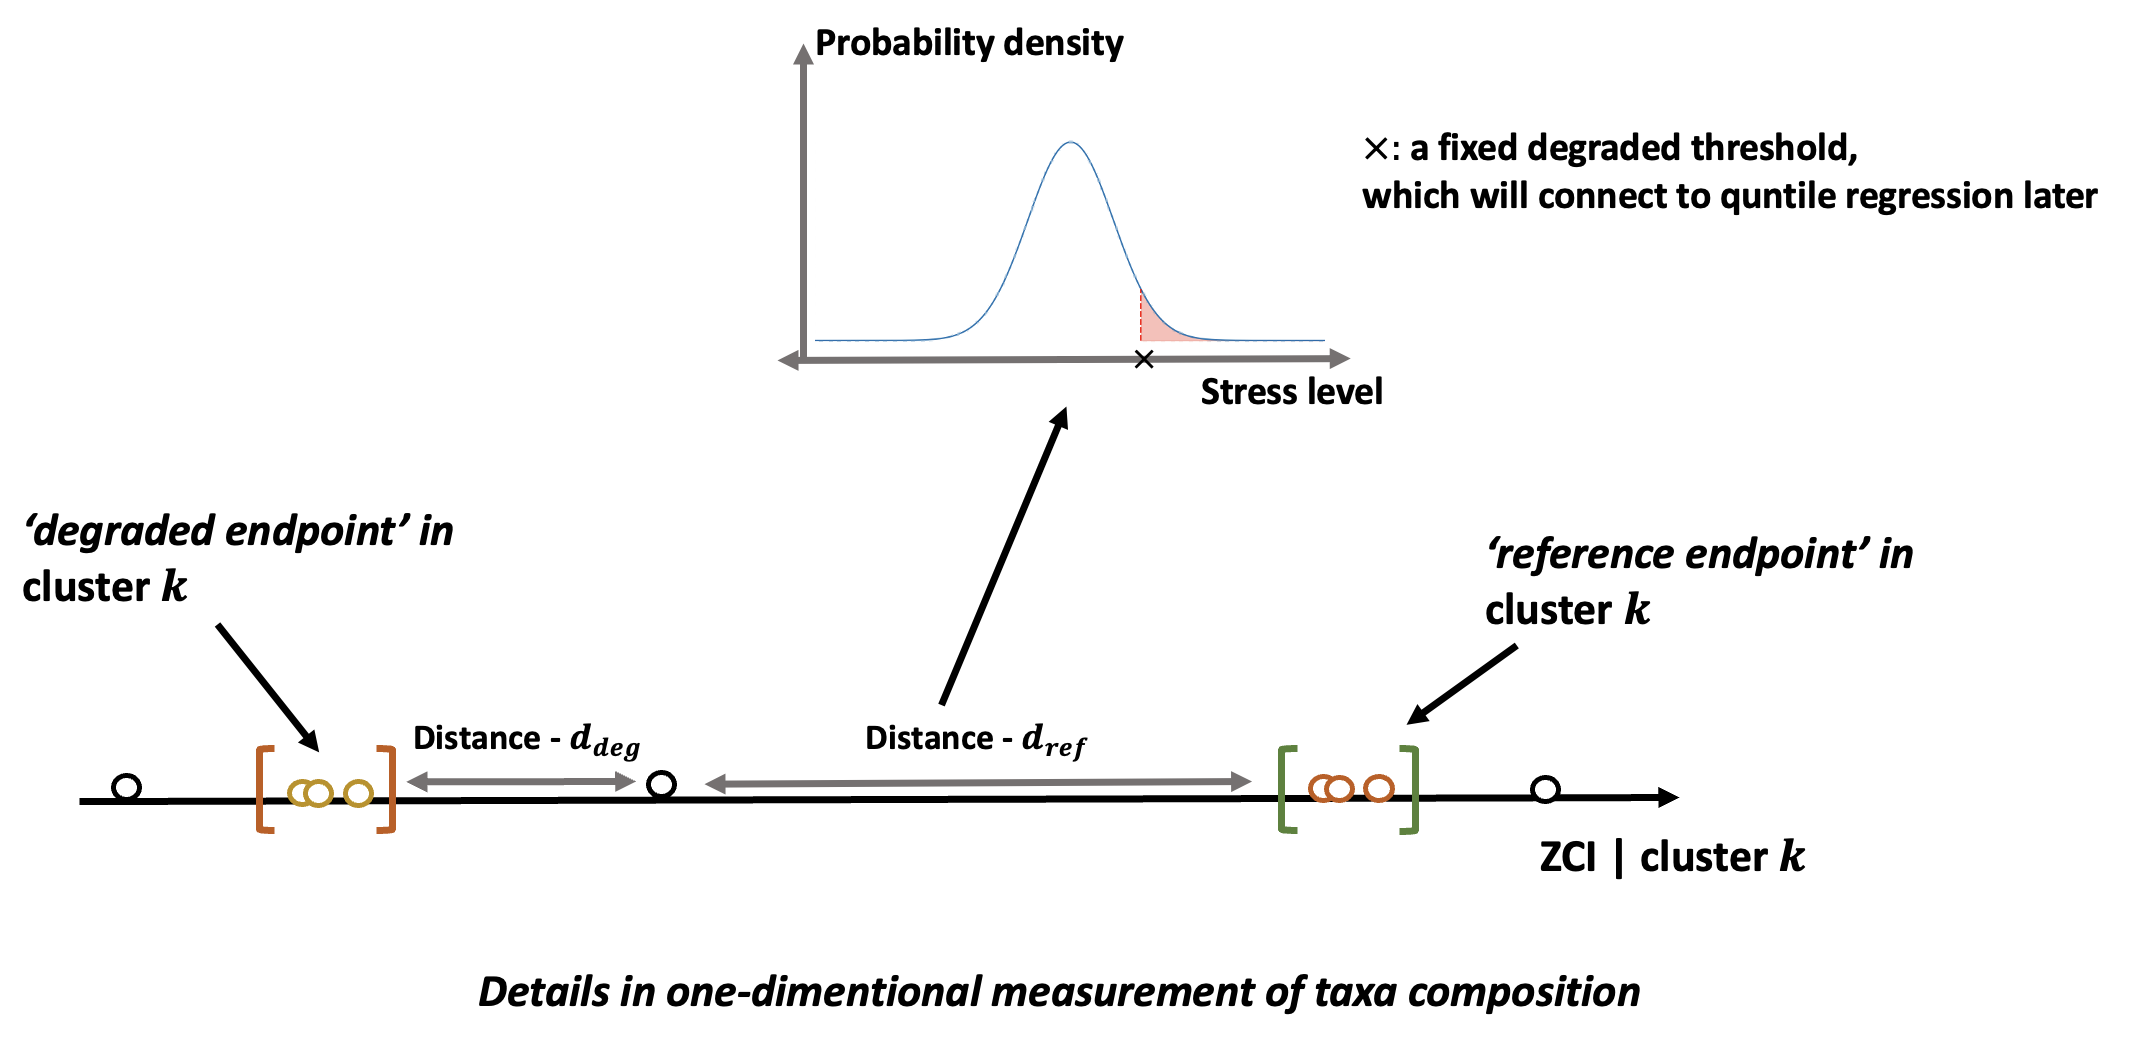
\includegraphics[width=\textwidth]{figures/p15_details_of_taxa_difference_in_1dimention.png}
\end{figure}

\end{frame}

\begin{frame}
\frametitle{Details in the the one-dimensional taxa difference measurements}
% The true distribution of stress level is unknown, and may not be necessary to know and some critical values are more 
% meaningful.

\begin{figure}
\centering
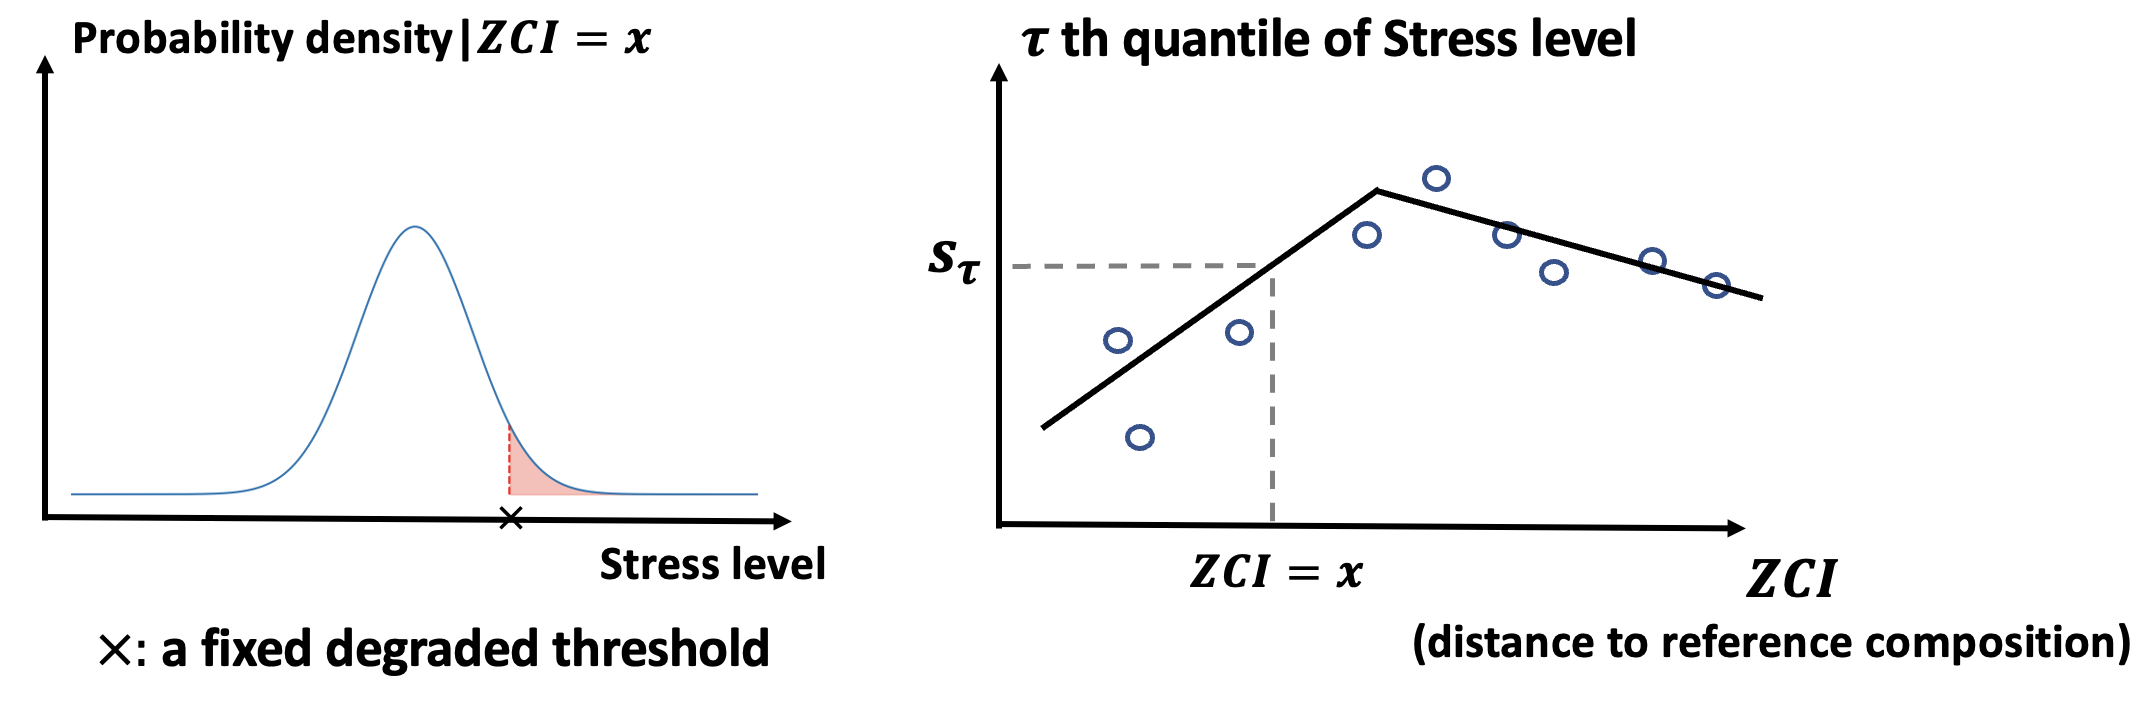
\includegraphics[width=.9\textwidth]{figures/p16_degraded_threshold_and_quantile_regression.png}
\end{figure}

% \vspace*{-1cm}
$s_{\tau}$: the right predicted $\tau$ quantile of the stress level that is equal to the threshold value.

The higher the $\tau$ parameter required to reach the threshold value, the safer it is to reject 'not degraded' decision.

$\tau = 1$: \textbf{all samples} are less than the threshold and support to say 'not degraded';
$\tau \approx 0$: \textbf{only one or no sample} is less than the threshold and supports to say 'not degraded'

\end{frame}

\begin{frame}
\frametitle{Recap of the value-based measurements on the stress level and taxa composition}

\begin{figure}
\centering
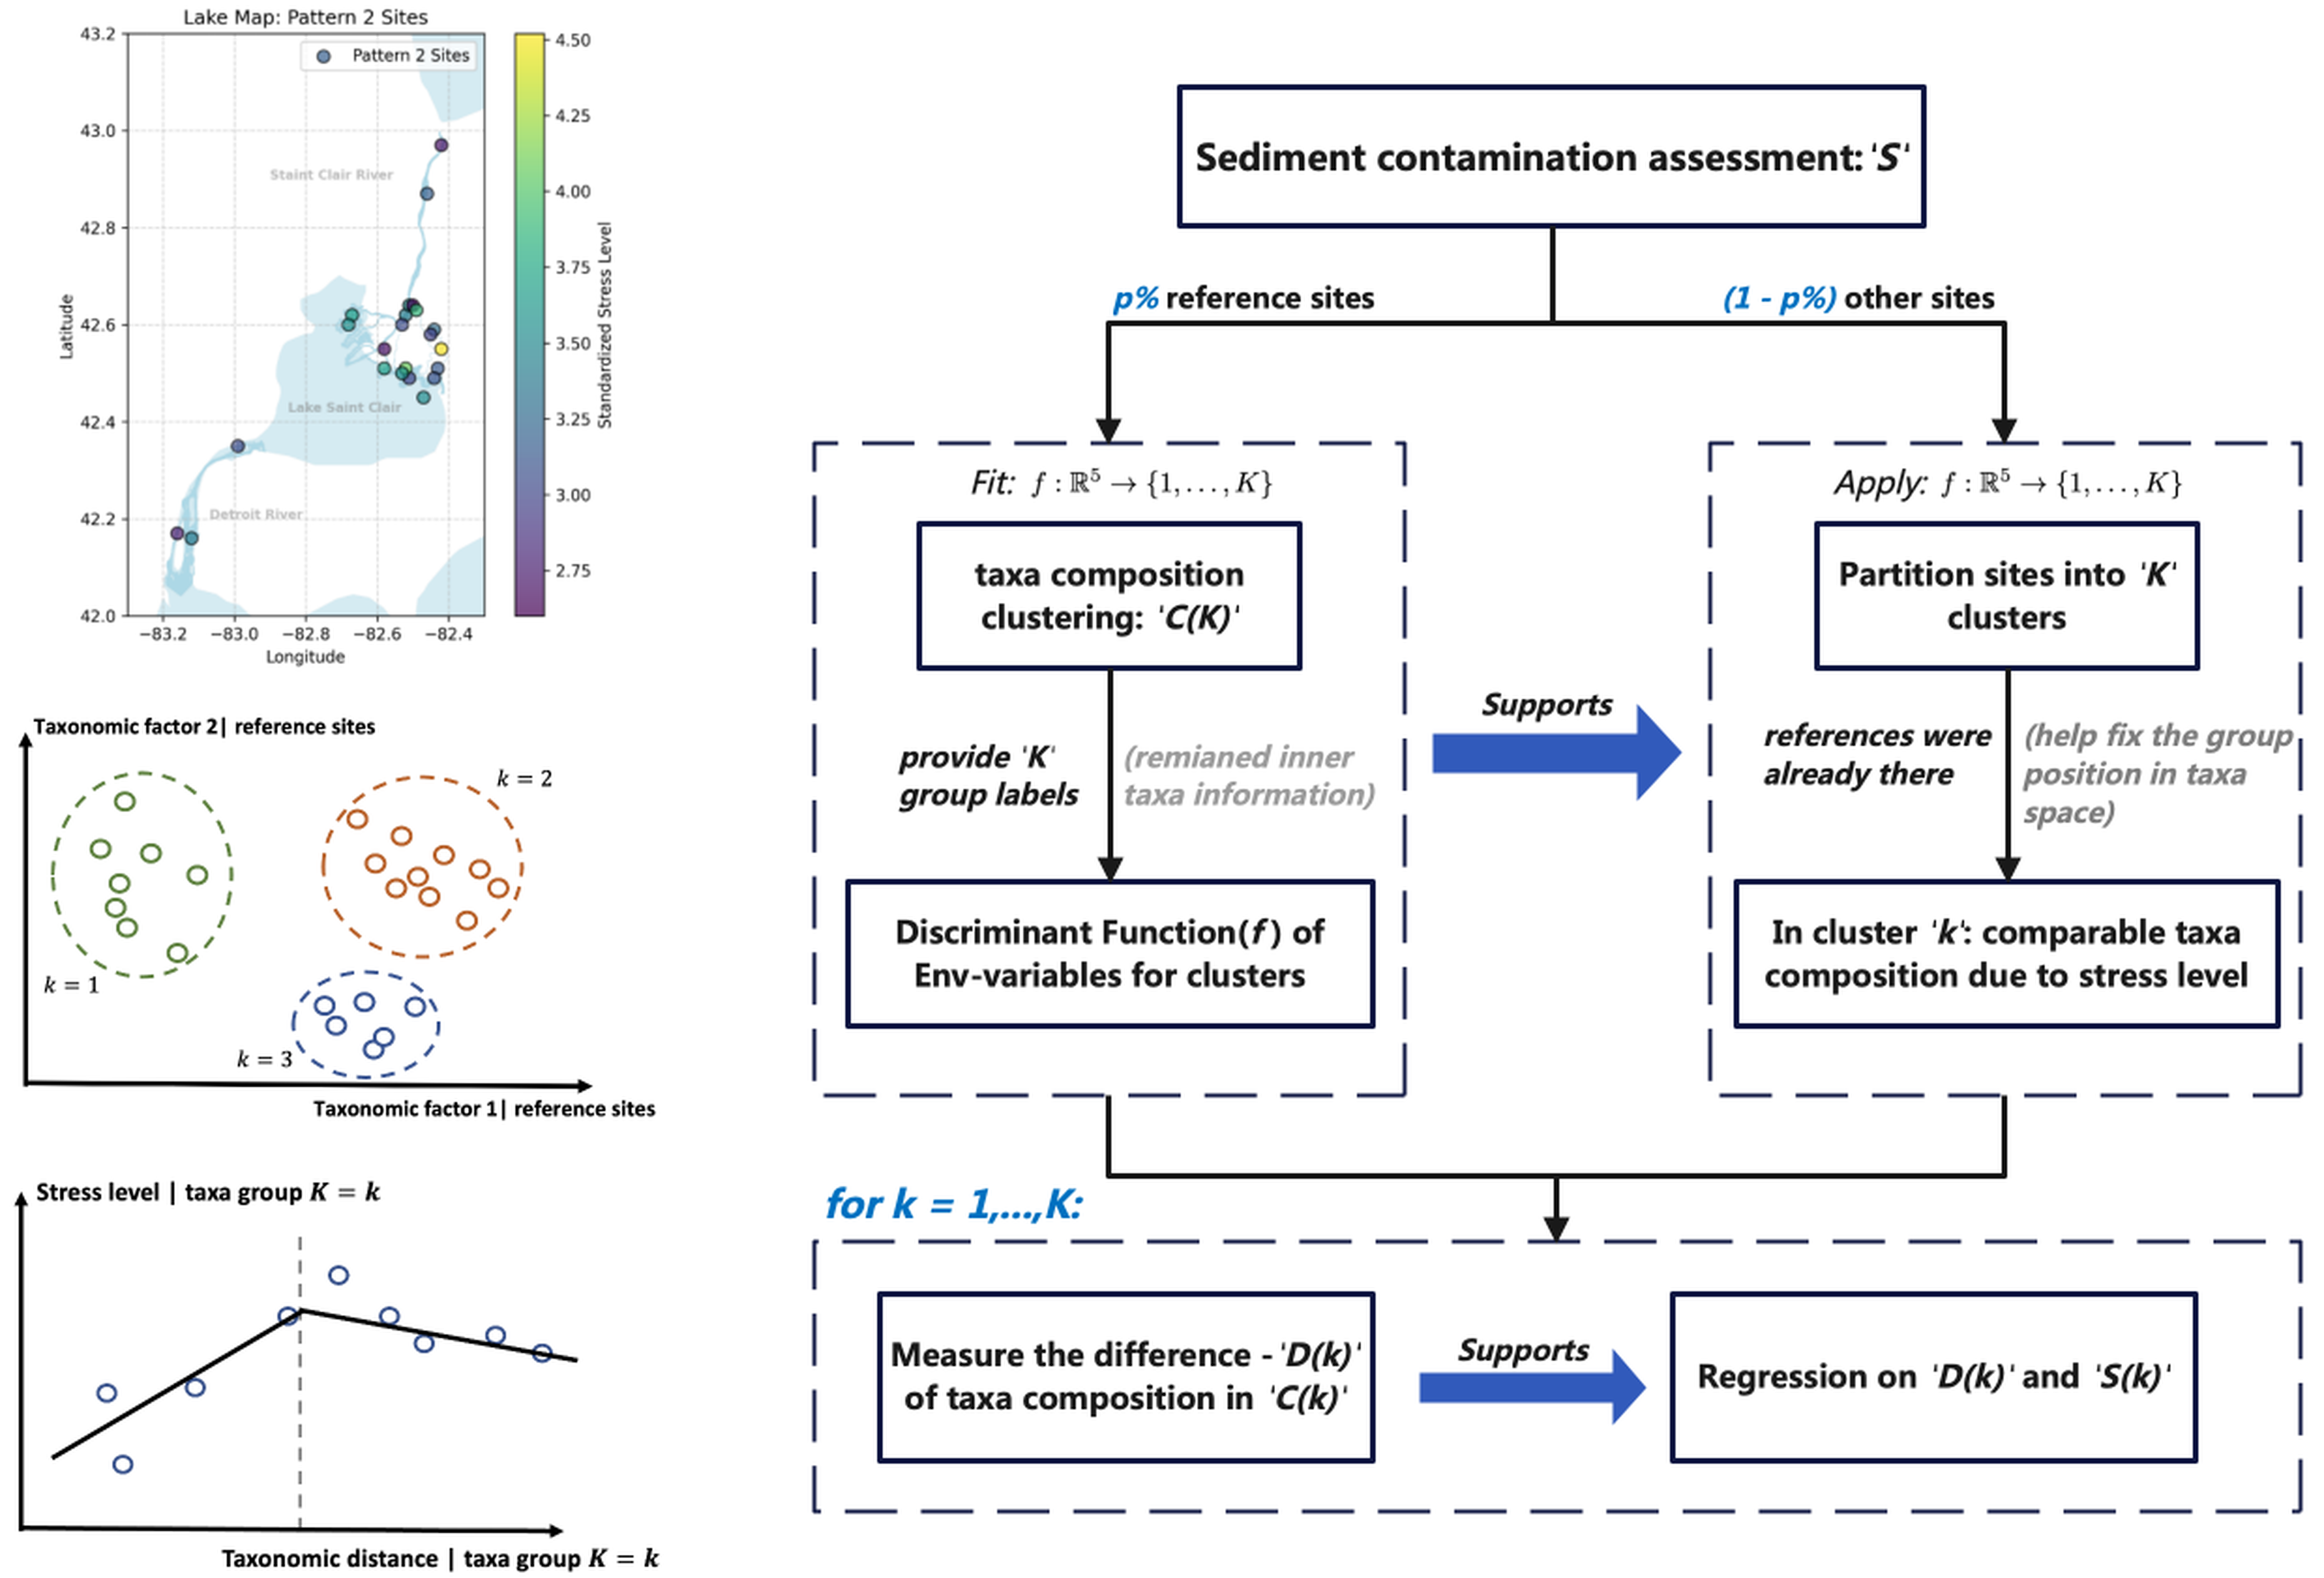
\includegraphics[width=\textwidth]{figures/workflow_of_general_workframe_part1.png}
\end{figure}

\end{frame}

\begin{frame}
\frametitle{From value-based measurements to vector-based measurements}

A value-based measurement, \(\mathcal{F}: R^p \to R\), sacrifices much information in the raw data, even though it 
carries more information than any single raw data column.

Sacrificing some simplicity, using a vector-based measurement, \(\mathcal{F}: R^p \to R^t (t < p)\),
can preserve more information to improve the inference accuracy.

In regression view, it transits from a simple regression to a multivariate regression.

\end{frame}

\begin{frame}
\frametitle{Reference sites in vector-based taxa composition measurements}
For \(k = 1, ..., K\):

\begin{figure}
    \centering
    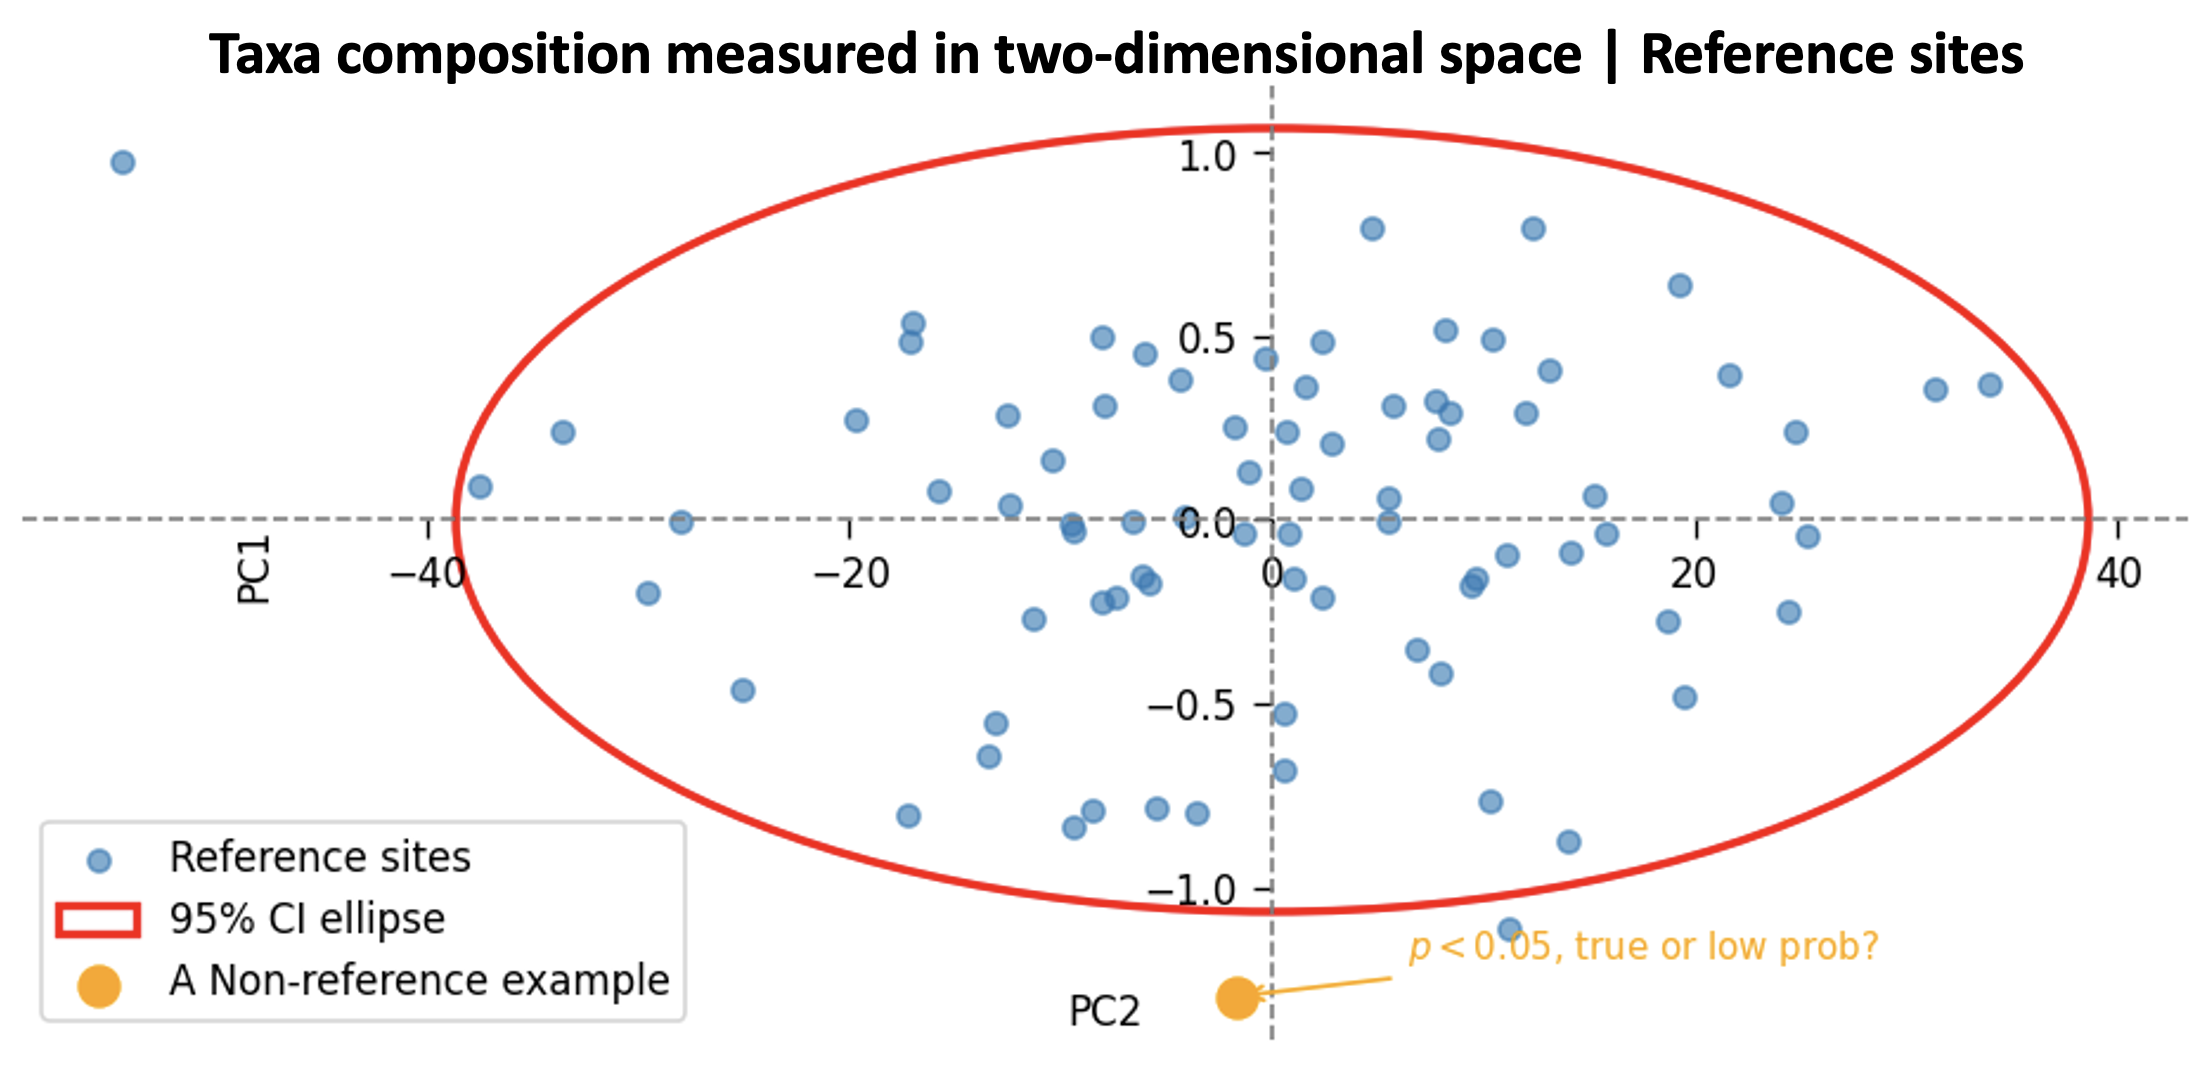
\includegraphics[width=\textwidth]{figures/p17_reference_area_in_2dimensional.png}
\end{figure}

\end{frame}

\begin{frame}
\frametitle{All sites in vector-based taxa composition measurements}
For \(k = 1, ..., K\):
\begin{figure}
    \centering
    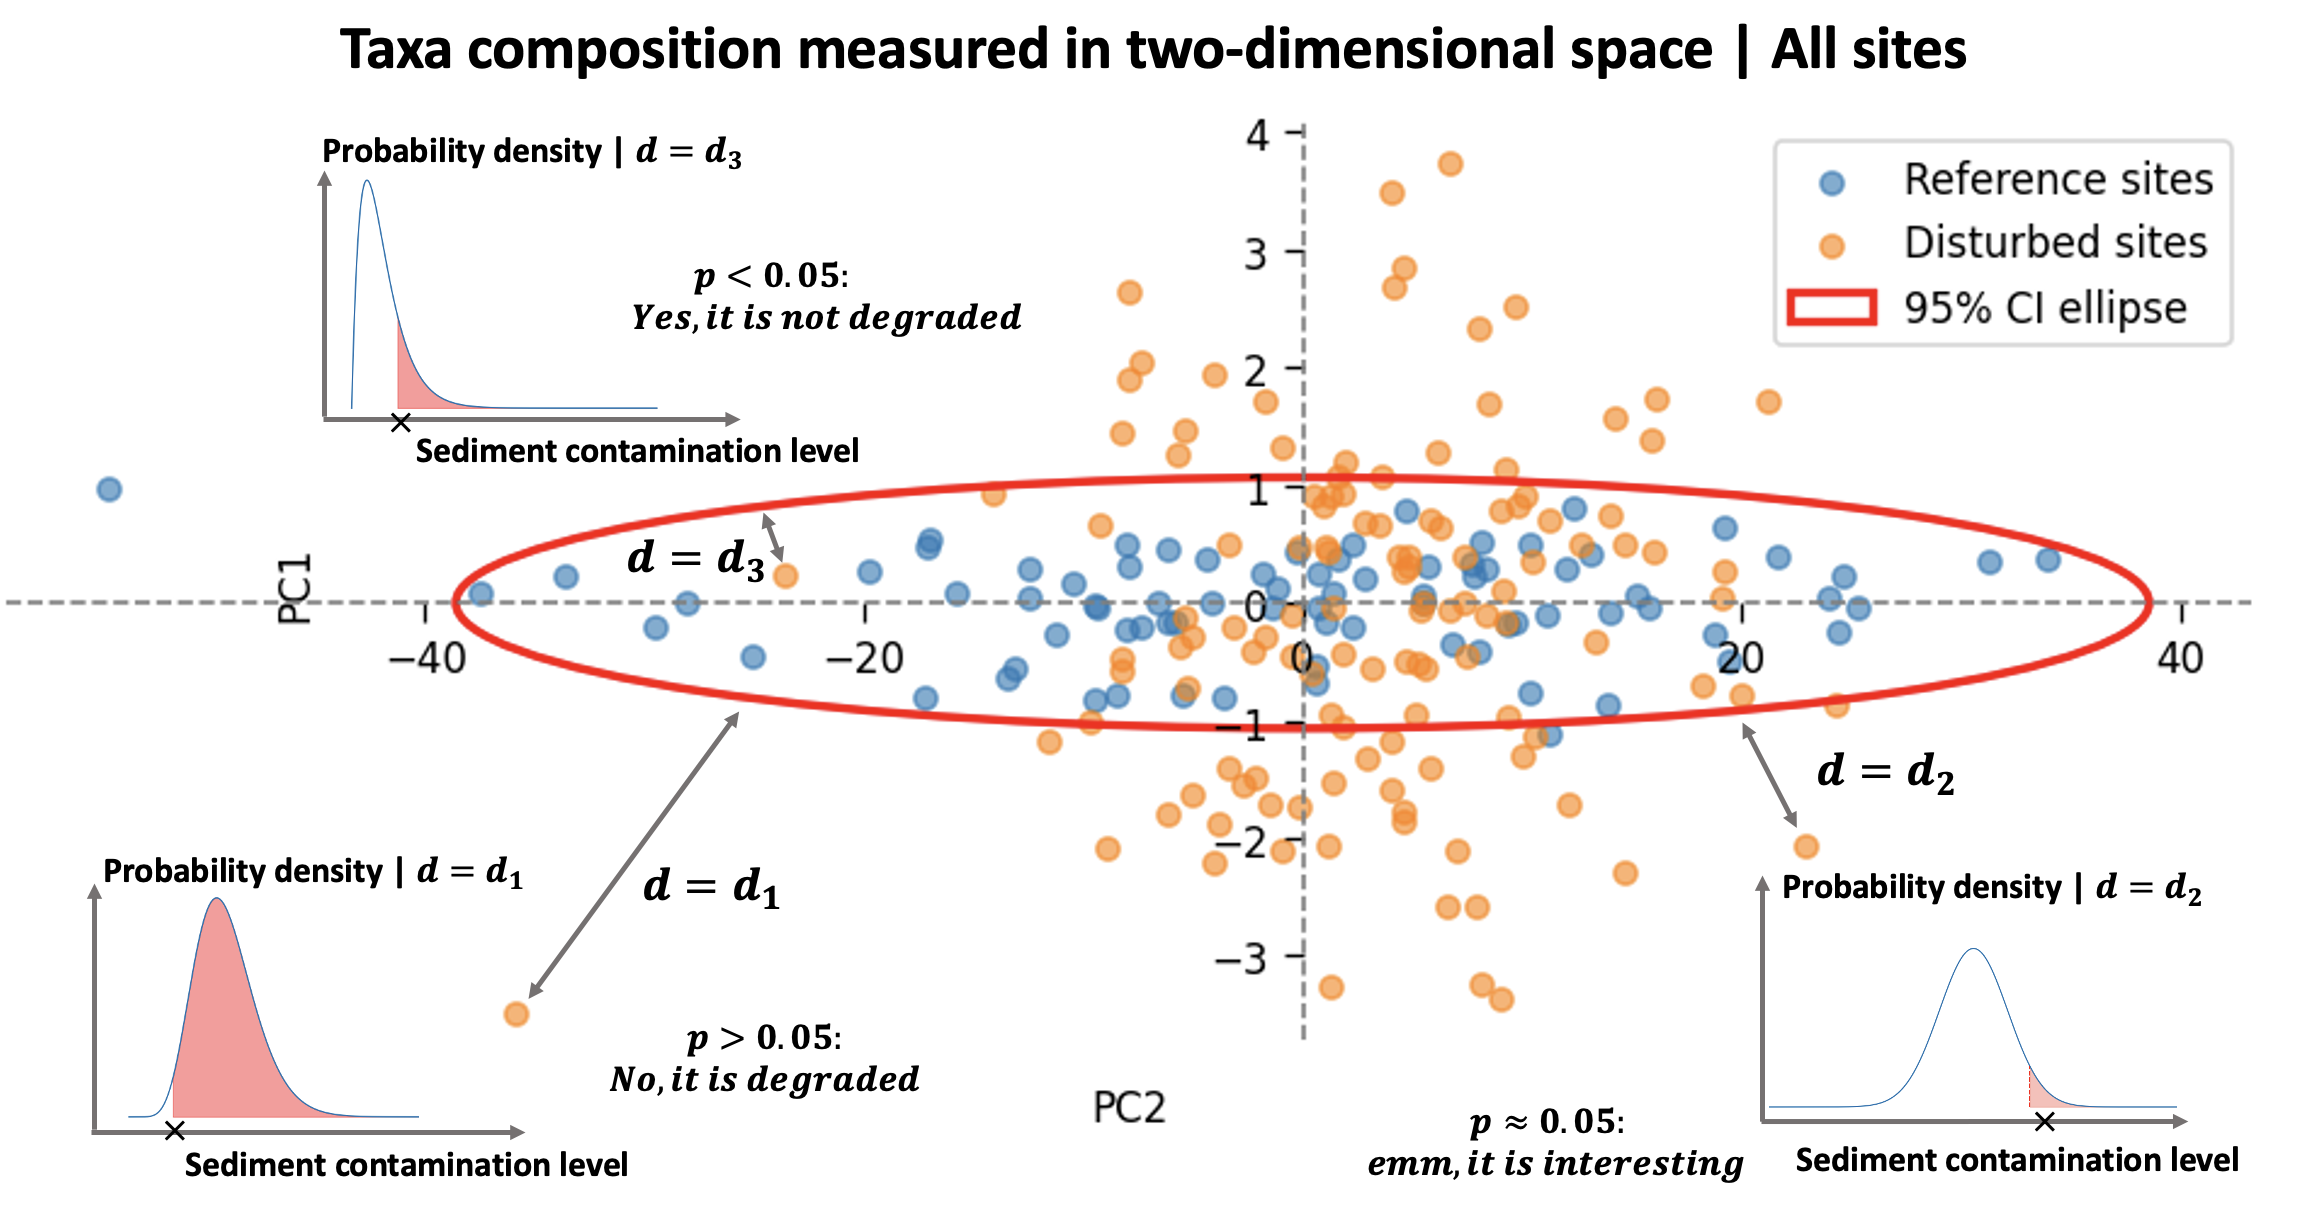
\includegraphics[width=\textwidth]{figures/p18_all_sites_in_2dimensional.png}
\end{figure}

\end{frame}

\begin{frame}
\frametitle{A hypothetically improved 2-dimensional taxa composition measurements}
For \(k = 1, ..., K\):
\begin{figure}
    \centering
    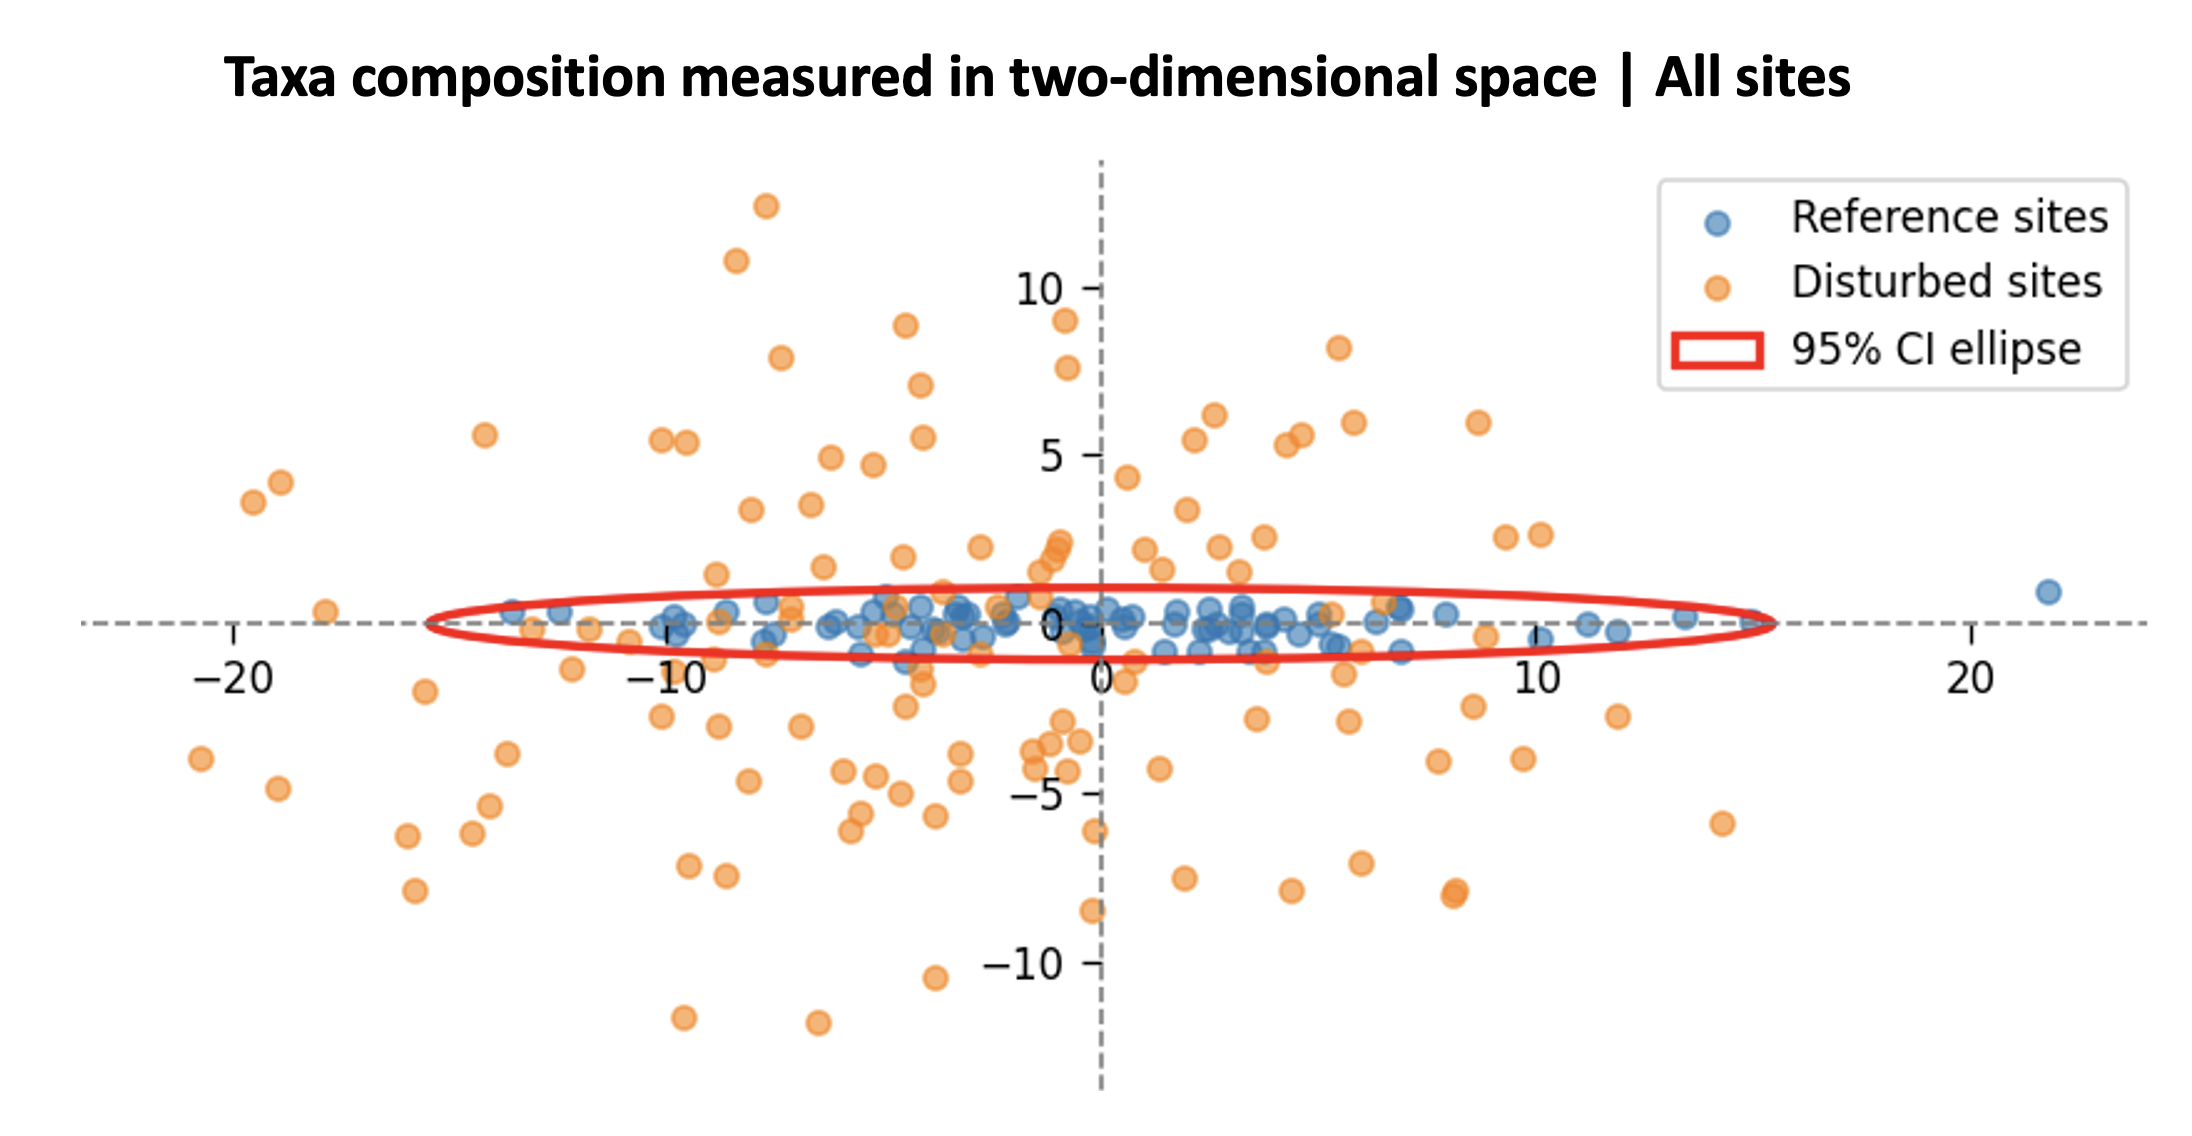
\includegraphics[width=\textwidth]{figures/p19_improved_2dimensional_measurements.png}
\end{figure}

\end{frame}

\begin{frame}
\frametitle{Additional techniques to enhance the process}

\begin{itemize}
    \item Supervised learning relevant methods to improve the discriminant function and quantile regression.
    \item Unsupervised learning relevant methods to improve the clustering of taxa composition.
    \item Synthetic data generation to partially counter the data scarcity problem.
\end{itemize}

\end{frame}

\begin{frame}
\frametitle{Potentially core tasks and challenges}

\begin{itemize}
    \item How to define and conduct the measurements of stress level and taxa composition?
    \item How to balance the correlation and respective interpretability of the 
    measurements? Is it possible to give up the all interpretability of taxa composition and 
    only measure it in the perspective of stress level? (maybe not good)
    \item Stress level assessment is the foundation influencing all following tasks,
    how to ensure its accuracy and reliability?
\end{itemize}

\end{frame}

\begin{frame}
\frametitle{Programming framework and pipeline design}

Assuming there are \(t\) acceptable methods in each stage, they do not influence our 
interpretation to the whole process, but they do influence the model performance 
(the distance measurements in the taxa composition space).
One way to find the best combination can be:

\begin{figure}
\centering
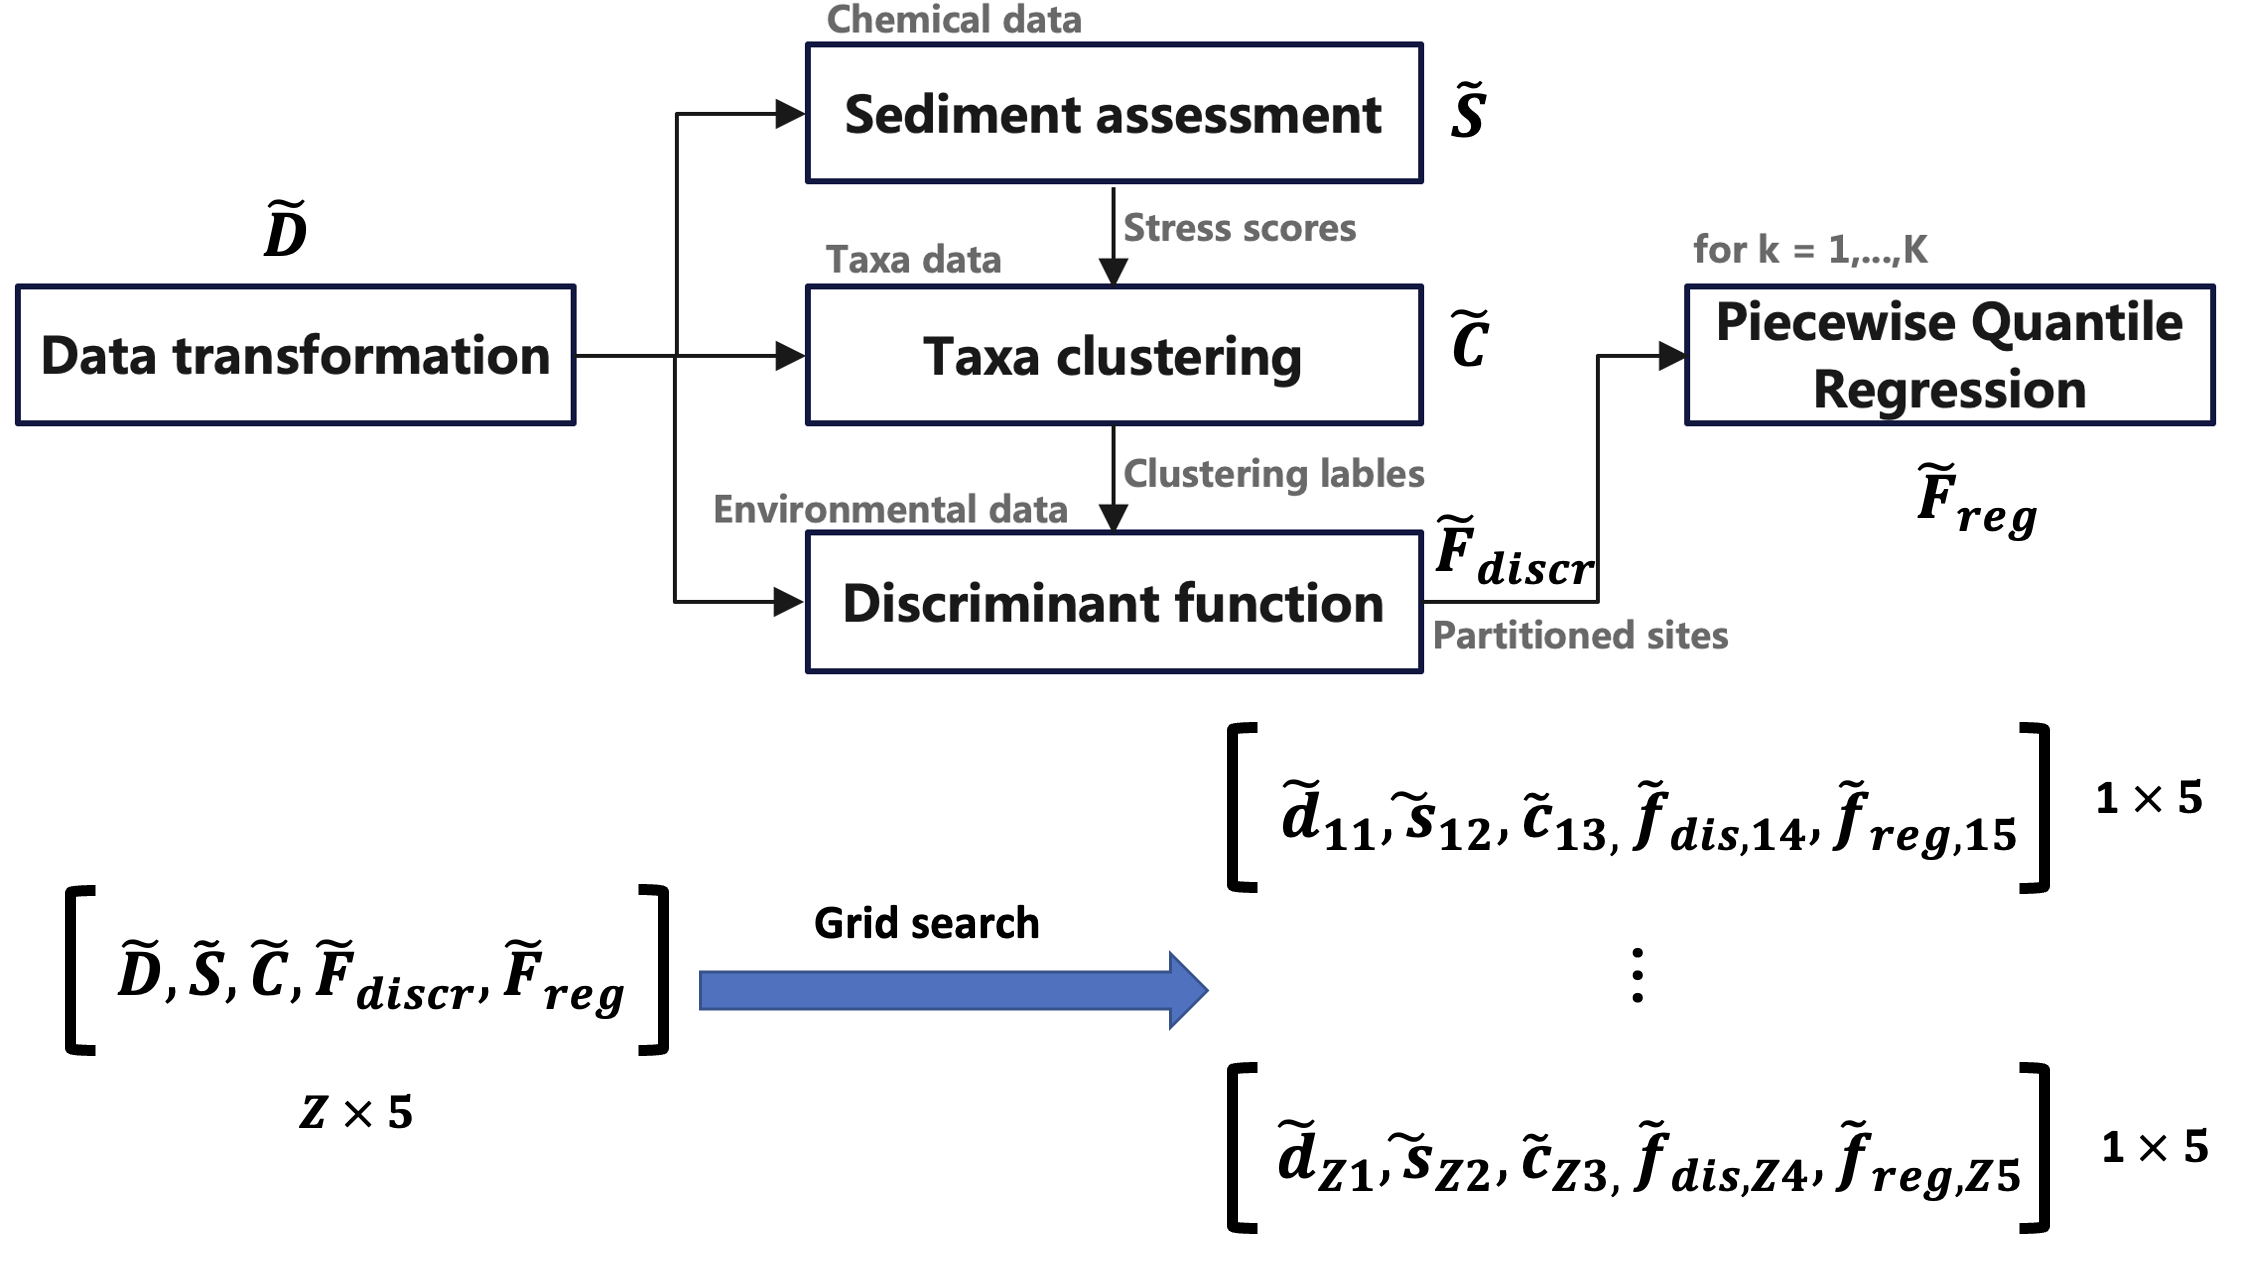
\includegraphics[width=\textwidth]{figures/p22_programing_pipeline.png}
\end{figure}

\end{frame}

\begin{frame}
\centering
\huge{Thank you!\\[1em]Questions?}
\end{frame}



\end{document}